\documentclass[]{article}
\usepackage{amsmath}
\usepackage{amsthm}
\usepackage{amssymb}
\usepackage{graphicx}
\usepackage{float}
\usepackage{listings}
\usepackage{caption}
\usepackage{subcaption}
\usepackage[round]{natbib}
\bibliographystyle{unsrtnat}

%\usepackage{multicol}
%\usepackage{bm}
%\usepackage{physics}

% this just sets up the page size and margins
\setlength{\topmargin}{0pt}
\setlength{\oddsidemargin}{0pt}
\setlength{\evensidemargin}{0pt}
\setlength{\textwidth}{6.5in}
\setlength{\textheight}{8.5in}
\setlength{\headheight}{0pt}

%%%%%%%%%%%%%%%%%%%%%%%%%%%%%%%%%%%%%%%%%%%%%%%%
%
%  This is all the stuff for Python code snippets
%
\DeclareFixedFont{\ttb}{T1}{txtt}{bx}{n}{10} % for bold
\DeclareFixedFont{\ttm}{T1}{txtt}{m}{n}{10}  % for normal
% Custom colors
\usepackage{color}
\definecolor{deepblue}{rgb}{0,0,0.5}
\definecolor{deepred}{rgb}{0.6,0,0}
\definecolor{deepgreen}{rgb}{0,0.5,0}

\setcounter{MaxMatrixCols}{15}

% Python style for highlighting
\newcommand\pythonstyle{\lstset{
		language=Python,
		basicstyle=\ttm,
		morekeywords={self},              % Add keywords here
		keywordstyle=\ttb\color{deepblue},
		emph={MyClass,__init__},          % Custom highlighting
		emphstyle=\ttb\color{deepred},    % Custom highlighting style
		stringstyle=\color{deepgreen},
		frame=tb,                         % Any extra options here
		showstringspaces=false,
		tabsize=4
}}

% Python environment
\lstnewenvironment{python}[1][]
{
	\pythonstyle
	\lstset{#1}
}
{}

% Python for inline
\newcommand\pythoninline[1]{{\pythonstyle\lstinline!#1!}}

%%%%%%%%%%%%%%%%%%%%%%%%%%%%%%%%%%%%%%%%%%%%%%%%%


\newcommand{\mpc}{MPC}
\newcommand{\nmpc}{NMPC}
\newcommand{\pdiff}{P_{\Delta}}
\newcommand{\pavg}{\overline{P}}
\newcommand{\R}{\mathbb{R}}
\newcommand{\casadi}{CasADi}
\newcommand{\dompc}{{\bf do-mpc}}

\title{Comparison of Direct Methods for NMPC  Applied to  a Thrust Vector Drone}
\author{Izzy Mones and Heidi Dixon}
%\date{}

\begin{document}
\maketitle
	
\section*{Introduction}	
	This paper is part of a larger project inspired by the small-scale rocket prototype presented by \cite{TVCDrone} which aims to study thrust vector control (TVC) and vertical takeoff and landing (VTOL) using a gimballed-thrust rocket prototype. 
	VTOL milestones like NASA's Lunar Landing Research Vehicle (LLRV) which allowed Apollo astronauts to practice lunar landings, McDonnell Douglas’s DC-X (Delta Clipper), and SpaceX's Falcon 9 landings, and the planned Artemis III mission that aims to land and return astronauts from the moon illustrate the value of propulsive VTOL with TVC. 	
	About the upright hover equilibrium, vertically flying rockets are open-loop unstable in attitude. They have highly nonlinear, coupled dynamics, and require fast control algorithms that respond quickly to disturbances and sensor noise. Unfortunately, validating control techniques on full-scale rockets is prohibitively costly and high-risk. There is a need for inexpensive test vehicles that allow experimentation with rocket guidance, navigation, and control. 
	A gimballed-thrust drone with electric motors and propellers is a good choice for replicating rocket dynamics on a much smaller budget. A couple of low-cost designs have been proposed and implemented  \citep{cheapTVC}, \citep{TVCDrone}. The drone design by \cite{TVCDrone} allows experimentation with control algorithms for VTOL and TVC. We have designed a similar drone based on their images and design descriptions, and there remain many details and design choices to explore.

	Our drone implements TVC and VTOL using a nonlinear model predictive control (NMPC) algorithm \citep{nmpc}, allowing it to handle nonlinear rocket dynamics and manage constraints like gimbal angle range, servo rates, and thrust limits. NMPC optimizes control inputs across a finite time horizon at each time step. In this sense it optimizes a control sequence, allowing it to anticipate future control requirements. Revising the sequence at each time step allows it to respond to disturbances. The main downside of NMPC is its high computational load. NMPC solves a constrained Optimal Control Problem (OCP) that is transcribed into a finite dimensional nonlinear optimization problem (NLP) at every control step, and as a result it is much slower than simple control algorithms like proportional integral derivative (PID) controllers or linear quadratic regulators (LQR).
	There are a variety of ways to formulate an NMPC problem instance as a nonlinear programming problem. Different formulations may vary in their computation times and solution accuracy. The focus of this paper is experimenting with different choices of NLP formulations and evaluating their speed and accuracy.  Our goal is to run our control algorithm on a Raspberry Pi 5 at $50$ Hz so solution speed will be very important.
	{\em We  compare three approaches: a Runge-Kutta multiple-shooter method, an orthogonal collocation with Gauss-Radau nodes implemented in the {\bf do-mpc}  library \citep{do-mpc},  and a Chebyshev pseudospectral collocation approach. We compare the relative accuracy of these techniques and their relative efficiency.}

	

	
\section*{Thrust Vector Drone Equations of Motion}
	
	The system state $\vec{x}$ includes translational position $\vec{p} = [x, y,  z]$ and velocity $\vec{v} = [v_x, v_y, v_z ]$  in the world frame, the attitude represented as a unit quaternion $\vec{q} = [q_x, q_y,  q_z, q_w]$ and the angular velocity in the body frame $ \vec{\omega} = [\omega_x, \omega_y, \omega_z]$. The control variables include the two gimbal angles $\theta_1, \theta_2 $, the average thrust between the two propellers $\pavg$ and the differential thrust between the propellers $\pdiff$ to control the rotation about the body $z$ axis.
	\begin{gather*}
		\vec{x} =
		\begin{bmatrix}
			x & y & z & v_x & v_y & v_z & q_x & q_y & q_z & q_w & \omega_x & \omega_y & \omega_z
		\end{bmatrix}^T \\
		\vec{u} =
		\begin{bmatrix}
			\theta_1 & \theta_2 & \pavg & \pdiff
		\end{bmatrix}^T
	\end{gather*}
	The equations of motion are represented as a series of first-order vector differential equations:
	\begin{gather}
		\dot{\vec{p}}  = \vec{v}         \label{eqMotion1}	\\
		\dot{\vec{v}}  = \frac{1}{m}R(\vec{q})\vec{F_b}+\vec{g}  \label{eqMotion2} \\
		\dot{\vec{q}} = \frac{1}{2}Q(\vec{\omega})\vec{q}  \label{eqMotion3} \\
		\dot{\vec{\omega}} = I^{-1}\!\left(\vec{M_b} - \vec{\omega} \times (I\,\vec{\omega})\right) \label{eqMotion4}
	\end{gather}
	where $m$ is the mass of the drone and $\vec{g} = [0, 0, -9.81]^T$ is the acceleration due to gravity.
	\begin{figure}[H]
		\centering
		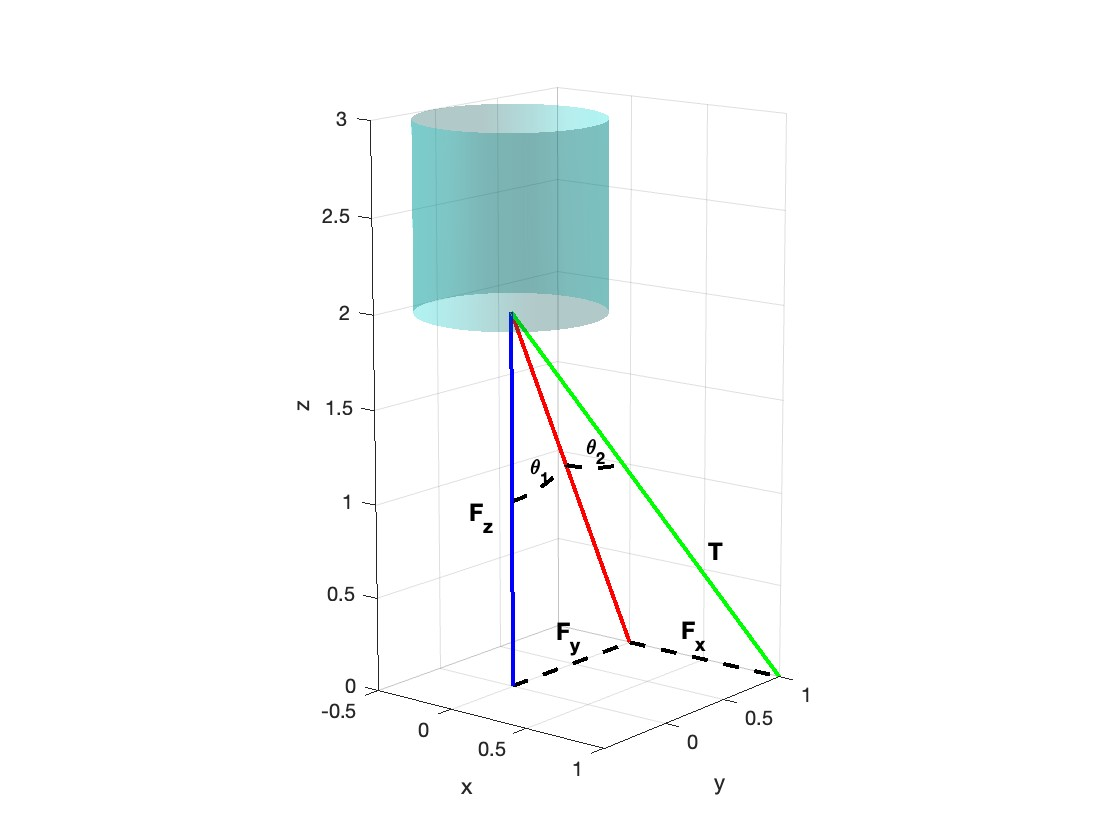
\includegraphics[width=0.7\textwidth]{figures/graph3d.jpg}
		\caption{Three-dimensional thrust decomposition for a 2-axis gimballed drone.}
		\label{fig:3dgraph}
	\end{figure}
	\begin{figure}[H]
		\centering
		\begin{subfigure}[b]{0.48\textwidth}
			\centering
			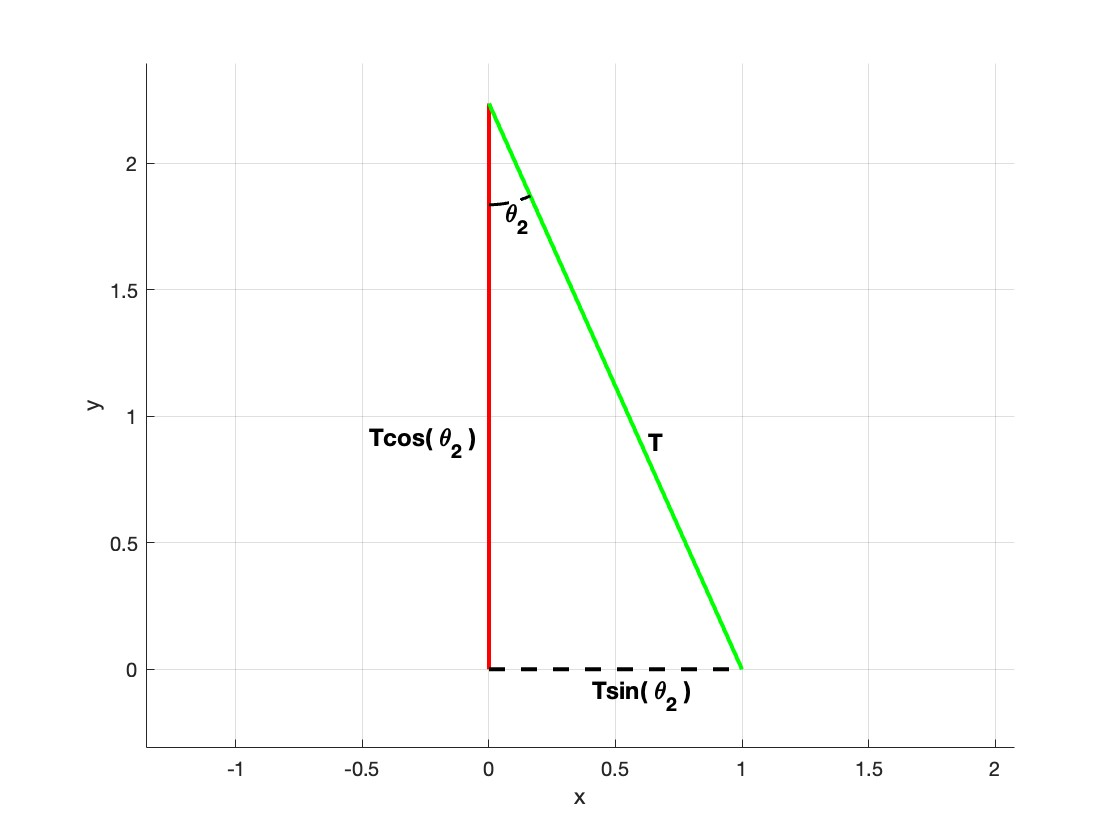
\includegraphics[width=\textwidth]{figures/graph2.jpg}
			\caption{Thrust decomposition in the inner gimbal axis plane.}
		\end{subfigure}
		\begin{subfigure}[b]{0.48\textwidth}
			\centering
			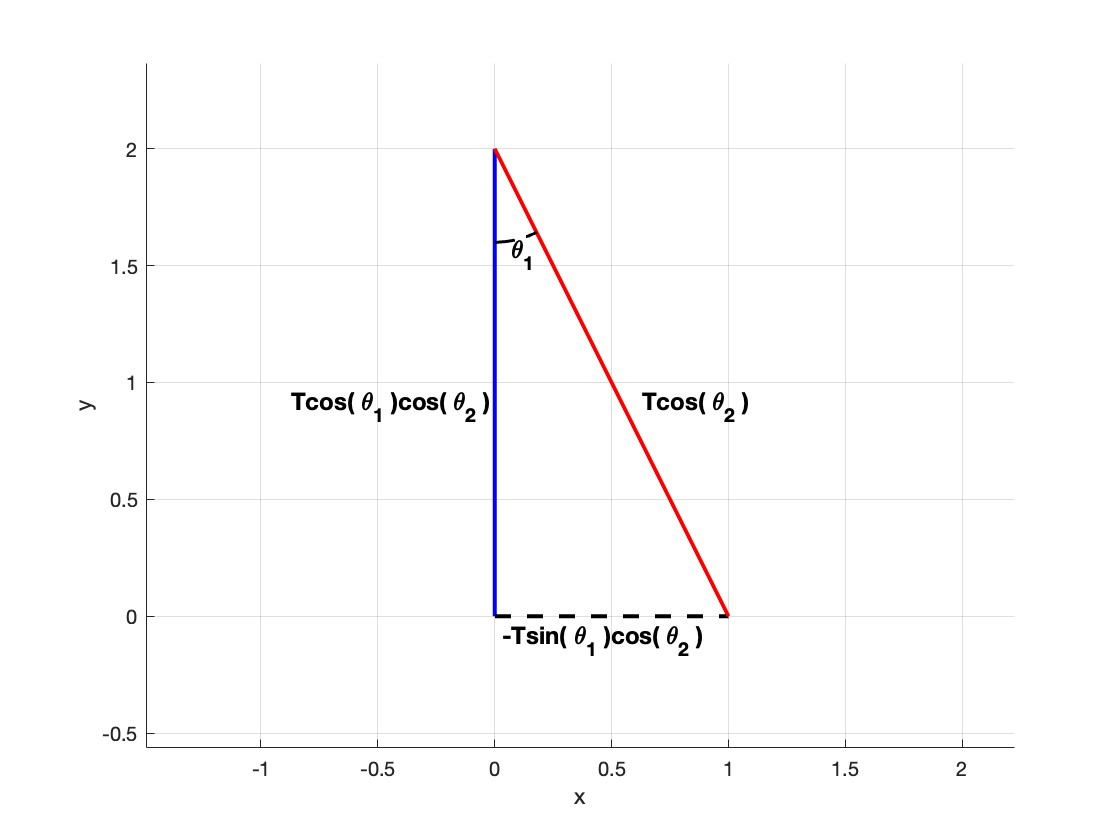
\includegraphics[width=\textwidth]{figures/graph3.jpg}
			\caption{Thrust decomposition in the x–z plane.}
		\end{subfigure}
		\caption{Two-dimensional thrust decompositions for a 2-axis gimballed drone.}
		\label{fig:3dDecomp}
	\end{figure}
	Using vector decomposition we can find the thrust vector in body coordinates in terms of the gimbal angles $\theta_1$ and $\theta_2$ and magnitude of the thrust $T$ acting on the drone.
\[
\vec{F_b} = T
\begin{bmatrix}
	\sin{\theta_2}  \\
	-\sin{\theta_1}\cos{\theta_2}  \\
	\cos{\theta_1}\cos{\theta_2}
\end{bmatrix}
\]
$\vec{M_z}$ is the moment about the body z axis due to differential thrust. 
        \[
	\vec{M_z} =
        \begin{bmatrix}
        0  \\
        0  \\
        M_z
        \end{bmatrix}
        \]
The body frame moment vector is the sum of the torque due to thrust vector acting through the moment arm and the torque generated by the differential thrust. $l$ is the length of the moment arm acting from the center of mass to the point $\vec{F_b}$ acts on the drone in body coordinates. 
        \[
	\vec{l} =
        \begin{bmatrix}
        0  \\
        0  \\
        -l
        \end{bmatrix}
        \]
        	 \[
        \vec{M_b} = \vec{l} \times \vec{F_b} + \vec{M_z}=       
        \begin{bmatrix}
        -lT\sin{\theta_1}\cos{\theta_2}  \\
        -lT\sin{\theta_2}  \\
	M_z
        \end{bmatrix}
        \]
The drone is designed to be symmetrical and the principal axes align with the body frame. The products of inertia vanish and inertia tensor can be written with only diagonal terms.
         \[
        I =
        \begin{bmatrix}
        I_{xx} & 0 &0 \\
        0 & I_{yy }& 0 \\
        0 & 0 & I_{zz}
        \end{bmatrix}
        \]
The body to world matrix is used to compute the force in world coordinates due to the body-centric thrust vector given the quaternion orientation.
        \[
        R(\vec{q}) =
        \begin{bmatrix}
        1 - 2(q_y^2 + q_z^2) & 2(q_x q_y - q_w q_z) & 2(q_x q_z + q_w q_y) \\
        2(q_x q_y + q_w q_z) & 1 - 2(q_x^2 + q_z^2) & 2(q_y q_z - q_w q_x) \\
        2(q_x q_z - q_w q_y) & 2(q_y q_z + q_w q_x) & 1 - 2(q_x^2 + q_y^2)
        \end{bmatrix}
        \]
The quaternion propagation matrix computes the change in quaternions given a set of angular velocities.
        \[
        Q(\vec{\omega}) =
        \begin{bmatrix}
        0 & \omega_z & -\omega_y & \omega_x \\
        -\omega_z & 0 & \omega_x & \omega_y \\
        \omega_y & -\omega_x & 0 & \omega_z \\
        -\omega_x & -\omega_y & -\omega_z & 0
        \end{bmatrix}
	\]
	The final extended dynamic equations are expressed as:
	\[
		\dot{x} = v_x
	\]
	\[
		\dot{y} = v_y
	\]
	\[
		\dot{z} = v_z
	\]
	\[
		\dot{v_x} = \frac{\sin{\theta_2} *T(1 - 2(q_y^2 + q_z^2))-\sin{\theta_1}\cos{\theta_2}*2T(q_x q_y - q_w q_z)+\cos{\theta_1}\cos{\theta_2}* 2T(q_x q_z + q_w q_y)}{m}
	\]
	\[
		\dot{v_y} =\frac{\sin{\theta_2} *2T(q_x q_y + q_w q_z)-\sin{\theta_1}\cos{\theta_2}*T(1 - 2(q_x^2 + q_z^2))+\cos{\theta_1}\cos{\theta_2}* 2T(q_y q_z - q_w q_x)}{m}+g
	\]
	\[
		\dot{v_z} = \frac{\sin{\theta_2} *2T(q_x q_z - q_w q_y-\sin{\theta_1}\cos{\theta_2}* 2T(q_y q_z + q_w q_x)+\cos{\theta_1}\cos{\theta_2}* T(1 - 2(q_x^2 + q_y^2))}{m}
	\]
	\[
		\dot{q_x} = \frac{\omega_z q_y-\omega_y q_z+ \omega_x q_w}{2}
	\]
	\[
		\dot{q_y} = \frac{-\omega_z q_x+\omega_x q_z+ \omega_y q_w}{2}
	\]
	\[
		\dot{q_z} =  \frac{\omega_y q_x-\omega_x q_y+ \omega_z q_w}{2}
	\]
	\[
		\dot{q_w} =  \frac{-\omega_x q_x - \omega_y q_y - \omega_z q_z}{2}
	\]
	\[
		\dot{\omega_x} = \frac{-lT\sin{\theta_1}\cos{\theta_2}-\omega_y\omega_zI_{zz} + \omega_y\omega_zI_{yy}}{I_{xx}}
	\]
	\[
		\dot{\omega_y} = \frac{-lT\sin{\theta_2}-\omega_x\omega_zI_{xx} + \omega_x\omega_zI_{zz}}{I_{yy}}
	\]
	\[
		\dot{\omega_z} =  \frac{M_z -\omega_x\omega_yI_{yy} + \omega_x\omega_yI_{xx}}{I_{zz}}
	\]
Note that these equations use the variable $T$ representing the magnitude of the thrust vector acting on the drone. 
The actual control variables are defined as the average $\pavg$ and difference $\pdiff$ between the two propeller thrust values $T_1$ and $T_2$. 
	\[
		\pavg =\frac{T_1+T_2}{2}
	\]
	\[
		\pdiff =T_1-T_2
	\]
$T_1$ and $T_2$ denote the normalized brushless motor command signals, ranging from 0 (no throttle) to 1 (full throttle).
	\[
		T_1 = \pavg + \pdiff/2
	\]
	\[
		T_2 = \pavg - \pdiff/2
	\]
To map the average thrust command signal value to the actual thrust force value in Newtons used in the thrust-vector decomposition a second-order polynomial fit is experimentally determined. Similarly, a linear relationship is used to map the differential thrust to the moment about the body frame z axis.
	\[
		T = a\pavg^2+b\pavg+c
	\]
	\[
		M_z = d I_{zz} \pdiff
	\]

	


\section*{Nonlinear Model Predictive Control (NMPC)}

	Model predictive control (\mpc) is a control algorithm that solves an optimization problem at each time step.
	An {\mpc} solution yields a series of control inputs over a finite time horizon, creating a {\em plan} of actions that can anticipate and adjust to future issues. For example, the optimal speed for a car at a given instance might change if the algorithm knew that it was entering a curve in the road in the next few time steps. The control values for the first step of the plan is applied to the system and then the plan is revised at the next time step, allowing the method to react to disturbances and noise. Nonlinear model predictive control (\nmpc) is a variant of {\mpc} that can handle nonlinear dynamics. 

	Generally, given a set of continuous time nonlinear differential equations $\dot{x} = f(x(t),u(t))$  and an initial state $x_0$, the finite horizon {\nmpc} optimization problem is
	\begin{align*}
		\min_{u(t)} \; & \int_{0}^{t_f} \ell(x(t),u(t))\,dt  \\
		\text{s.t.} \;\; & \dot{x} =  f(x(t),u(t)) \\
		& x(0) = x_0 
	\end{align*}
	The solution $u(t)$ is a real valued function that minimizes the cost function over time interval $[0, t_f]$. The constraints require that  $u(t)$ and $x(t)$ obey the system dynamics $\dot{x} =  f(x(t),u(t)) $ and the  initial state $x(0)$ must be equal to the current state $x_0$.   Given this framework, it is easy to add additional constraints that enforce system limitation such as minimum or maximum control values.

	 Equations (\ref{eqMotion1}-\ref{eqMotion4}) are strongly nonlinear, but can be linearized around the fixed point in which the drone is vertically balanced as in LQR and Linear {\mpc}.  However, the linearized equations quickly become inaccurate if the drone moves away from the fixed point by tilting or rotating.  Working directly with the nonlinear equations allows more accurate predictions of the drone behavior. The {\nmpc} framework also allows us to enforce the mechanical limitations of our thrust motors and gimbal servos.  Libraries like {\casadi} \citep{casadi} and {\dompc} \citep{do-mpc} make {\nmpc} easy to implement in practice.
 
 	An {\nmpc} instance for the thrust vector drone is a minimization problem of the form
	\begin{align}
	   \min_{u(t)} \; &  \int_{0}^{t_f} \ell(x(t),u(t))\,dt  \;+\; \phi(x_f) \label{nmpc:cost} \\
	   \text{s.t.} \;\; 	&  \dot{x} =  f(x(t),u(t))  \nonumber \\ 
	   				& x(0) = x_0 \nonumber \\
	   				&	-\theta_{max} \leq \theta_1 \leq \theta_{max} \label{nmpc:gimbal1} \\
	   				& 	-\theta_{max} \leq \theta_2 \leq \theta_{max} \label{nmpc:gimbal2} \\
	   				& 	T_{min}  \leq \pavg + \pdiff/2 \leq T_{max} \label{nmpc:thrust1} \\
	   				&    T_{min} \leq  \pavg - \pdiff/2 \leq T_{max} \label{nmpc:thrust2} \\
	   				&        0 \leq z. \label{nmpc:vert}
	  %	  &       T_{diff_{min}} \leq \pdiff \leq T_{diff_{max}} \label{nmpc:thrust3} \\
	  %	  & 	-\dot{\theta}_{max} \leq \dot{\theta}_1 \leq \dot{\theta}_{max} \\
	  %	  &  	-\dot{\theta}_{max} \leq \dot{\theta}_2 \leq \dot{\theta}_{max}\\ 
	\end{align}
	The cost function (\ref{nmpc:cost}) minimizes both the squared error between the current state $x(t)$ and the goal state $x_{ref}$ weighted by diagonal matrix $Q$ and the error between the current control $u(t)$ and the goal control $u_{ref}$ weighted by diagonal matrix $R$. 
	\begin{equation*}
		\ell(x(t),u(t))= (x(t)-x_{ref})^T Q (x(t)-x_{ref}) + (u(t)-u_{ref})^T R (u(t)-u_{ref}) 
	\end{equation*}
	We also add a terminal cost 
	\begin{equation*}
		\phi(x_f) = (x(t_f)-x_{ref})^T Q_f (x(t_f)-x_{ref})
	\end{equation*}
	The problem instance also enforces minimum and maximum gimbal angles (\ref{nmpc:gimbal1},\ref{nmpc:gimbal2}), minimum and maximum values for each thrust motor (\ref{nmpc:thrust1}, \ref{nmpc:thrust2}) and restrictons on the drone's vertical height (\ref{nmpc:vert}).




\section*{NLP Formulations}

	To solve the continuous time optimal {\nmpc} instance it is formulated as a discrete time finite dimensional nonlinear problem (NLP) and solved by a standard NLP solver.  NLP solvers are well established, highly optimized methods that originated in the field of operations research. Unfortunately, despite the availability of efficient solvers for these problems, NLP solutions for {\nmpc} problem instances may be too slow to produce control inputs for a thrust vector drone which requires a fast response time. This is a prime drawback of {\mpc} and {\nmpc} algorithms over LQR and PID  methods which can be computed very quickly.
	Ideally, we'd like to run our control algorithm at $50$Hz on a Raspberry Pi 5.  To meet this timing restriction we need to build an {\nmpc} instance that can be solved efficiently. 

	An NLP problem over a finite set of decision variables $w$ has the form 
	\begin{align}
		\min_{w \in \R^n} \; &  F(w) \label{nlp:opt} \\
		\text{s.t.} \;\; & G(x_0, w) = 0 \label{nlp:equality} \\
		&	H(w) \leq 0 \label{nlp:inequality}
	\end{align}
	It has an optimization function (\ref{nlp:opt}),  a set of equality constraints (\ref{nlp:equality}) and a set of inequality constraints (\ref{nlp:inequality}).
	In practice, the distinction between equality and inequality constraints is moot since an equality constraint can be written as two inequality constraints  and  an inequality constraint can be written as an equality constraints with the introduction of a slack variable. 

	To turn our {\nmpc} problem into an NLP problem  the continuous time functions $x(t)$ and $u(t)$ are parameterized into a finite set of discrete variables over the control trajectory.  Then differential equations for the system dynamics are discretized using a numerical integration method.  There are a many ways to do this and the choices we make will affect the size of the problem, the speed at which it can be solved, and the accuracy of the numerical approximation. Typically there is a tradeoff between speed and accuracy.  
	Next we explore three different ways to formulate our {\nmpc} problem as an NLP and compare and contrast their ability produce viable control trajectories and their relative efficiency.  These three methods are in no way exhaustive. We chose to implement pseudospectral collocation because it was shown to be effective in an earlier paper on thrust vector drones \citep{TVCDrone} and we chose multiple shooting and orthogonal collocation because they were very easy to implement.


\subsection*{Multiple Shooting (with Runge–Kutta discretization)}
	For multiple shooting, we divide our time horizon into $N$ evenly spaced nodes $\{ t_0, t_1, \ldots, t_N \}$ of length $\Delta t$ and we make copies of our state $x_k$ and control $u_k$ variables for each time step.  The initial state is initialized to the current state
	\begin{equation*}
		x_0 - X_0 = 0.
	\end{equation*}
	Using the system dynamics $\dot{x} =  f(x(t),u(t))$ and Runge-Kutta within each time step $[t_k, t_{k+1}]$ we forward integrate our differential equations 
	\begin{eqnarray}
	 	k_1 & = & f(x_k, u_k, t_k), \nonumber \\[6pt] \nonumber 
	 	k_2 & = & f\!\left(x_k + \tfrac{\Delta t}{2} k_1,\, u_k,\, t_k + \tfrac{\Delta t}{2}\right), \\[6pt] \nonumber
	 	k_3 & = & f\!\left(x_k + \tfrac{\Delta t}{2} k_2,\, u_k,\, t_k + \tfrac{\Delta t}{2}\right), \\[6pt] \nonumber
	 	k_4 & = & f\!\left(x_k + \Delta t\, k_3,\, u_k,\, t_k + \Delta t\right), \\[10pt]
	 	x_{k+1} - \Big(x_k + \tfrac{\Delta t}{6}(k_1 + 2k_2 + 2k_3 + k_4)\Big) &=& 0, 
	 	\qquad k = 0,\dots, N-1. \label{eq:rkstate}
     \end{eqnarray}
     to create constraints (\ref{eq:rkstate}) that enforce the change of state between time steps.
        
	The cost function is defined to penalize deviation from reference state as well as deviation from reference control input. There is also a terminal cost that incentivizes long term stability by weighting the final state more heavily.
        \[
        x_r =
        \begin{bmatrix}
        0 & 0 & 0 & 0 & 0 & 0 & 0 & 0 & 0 & 1 & 0 & 0 & 0
        \end{bmatrix}^{\!T},
        \qquad
        u_r =
        \begin{bmatrix}
        0 & 0 & T_{\text{hover}} & 0
        \end{bmatrix}^{\!T}.
        \]
         \begin{equation}
         	 \sum_{k=0}^{N-1}  \Big[(x_k -  x_{r})^T Q (x_k - x_{r}) + (u_k -  u_{r})^T R (u_k - u_{r}) \Big] + (x_N -  x_{r})^T Q_f (x_N - x_{r})
         \end{equation}
	Constraints on gimbal angles and thrust motors are encoded by adding a copy of the appropriate inequalities at each time step. 	To improve performance of our multiple shooter method we implemented warm starts, shifting the previous solution forward one time step and using that as an initial guess for the problem at the current time step.
	
	Multiple shooting considers the state and control variables at every time step to be optimization variables so the full NLP vector is:
        \[
        \begin{bmatrix}
        x_0 & u_0 & x_1 & u_1 & ... & x_{N-1} & u_{N-1} & x_N
        \end{bmatrix}
        \]
	This can easily become computationally demanding for long horizons and high-dimensional systems. For a thrust vector drone system with a  horizon length of 100 time steps there are $13 * (100+1)+4*100=1713$ decision variables. While the number of variables is very high, the constraint matrix is typically very sparse since each constraint references only a small number of variables.

	Multiple shooting is easy to implement using {\casadi}.  There are very few choices to toggle in producing the best multiple shooting implementation. Outside of specific NLP solver settings, the main choices are the length of your time steps and the length of your horizon.   Working with a time step of $\Delta t = 0.02$ we found that time horizons with $N \leq 50$  often produced trajectories that were irregular or did not converge. An $50 \leq N \leq 80$ produced mostly smooth graphs that converged however the convergence was a bit slow.  An $N \geq 80$ seemed to produce good quality graphs that converged promptly. However, our goal for all implementations is to have a horizon of $2$ seconds. 
	

	

\subsection*{Orthogonal Collocation using {do-mpc}} 
Of all the methods we implemented, orthogonal collocation was the easiest. We used the open source {\bf do-mpc} Python library for model predictive control  \citep{do-mpc}   which implements MPC and NMPC using orthogonal collocation with Radau nodes.
The {\bf do-mpc} library is ideal for prototyping  MPC and NMPC algorithms and requires minimal understanding of MPC and no understanding of orthogonal collocation to build functioning algorithms.

Need to discuss our cost function and how to encode servo and thrust minimum and maximums.  We should note that with do-mpc you don't need to know any of this because the NLP constraints are generated automatically from the system dynamics. Warm starts are done automatically in do-mpc. cost function and other constraints are entered using continuous model variables and do-mpc adapts them to the chosen trajectory variables. You can specify degree of collocation and time step size.

Orthogonal collocation is a local method that divides the time horizon into finite elements and fits polynomials to each interval. The dynamics are enforced throughout each interval at a set of $K+1$ Gauss-Radau nodes: the $K$ interior nodes, which are the roots of a Jacobi polynomial $P_K^{(\alpha,\beta)}$ of degree $K$, and one additional endpoint node, in this case the right endpoint, $\tau=1$. The Jacobi parameters $\alpha$ and $\beta$ determine the distribution of nodes throughout the interval, and a right-Radau formulation corresponds to $\alpha=1$, $\beta=0$.

\[
\gamma_0=1,  \qquad \gamma_j = \gamma_{j-1} \frac{(K-j+1)(K+j+\alpha+\beta)}{j(j+\beta)}, \qquad j = 1,\ldots,K
\]
When $P_K$ are the Gauss-Jacobi polynomials:
\[
P_K^{(\alpha, \beta)}(\tau) = \sum_{j=0}^{K}(-1)^{K-j}\gamma_j\tau^j
\]

Lagrange polynomials, $\ell_j(\tau)$, are used to interpolate the state trajectory $z^K(\tau)$:
\[
\ell_j(\tau)=\prod_{\substack{m=0 \\ m\neq j}}^{K}\frac{\tau-\tau_m}{\tau_j-\tau_m}
\]        
\[
z^K(\tau)=\sum_{j=0}^{K}z_{ij}\ell_j(\tau)
\]

By differentiating the state trajectory and equating it with the dynamics s$\dot{x} =  f(x(t),u(t))$, a dynamics constraint is formed:
\[
h_i=t_{i}-t_{i-1}
\]
\[
\sum_{j=0}^K z_{ij}\frac{d\ell_j(\tau_k)}{d\tau}=h_if(z_{ik},t_{ik}), 
\qquad k=1,\dots,K.
\]
Continuity constraints are used to fit an interval polynomial's endpoint with the first point of the next interval. There are two additional continuity constraints for enforcing the overall horizon's start and endpoint continuity.
\[
z_{i+1,0}=\sum_{j=0}^{K}\ell_j(1)z^{ij}
\]
\[
z_f=\sum_{j=0}^{K}\ell_j(1)z^{Nj}, \qquad z_{1,0} = z_0
\]
The continuous Bolza cost function is defined as:
\[
\substack {min \\ {x(t), u(t)}}J=\Phi(z(t_f),t_f) + \int_{t_0}^{t_f}L(z(t),u(t),t)dt
\]
Where $\Phi(z(t_f)$ is the Mayer term or terminal cost and $L(z_{ik},u_{ik},t_{ik})$ is the running cost. We then use a change of variables to convert from t to $\tau$. Using the general Gaussian Quadrature rule, we can substitute a quadrature sum of the cost at each given node for the integral of the running cost over the interval.
\[
h_i=t_{i}-t_{i-1} \qquad t=t_{i-1} + h_i\tau \qquad dt= h_i d\tau
\]
\[
\int_{t_0}^{t_f} L(z(t),u(t),t)dt = \sum_{i=1}^N \int_{t_{i-1}}^{t_i} L(z(t),u(t),t)dt=\sum_{i=1}^N h_i \int_{0}^{1} L(z(t_{i-1} + h_i\tau),u(t_{i-1} + h_i\tau),t_{i-1} + h_i\tau) d\tau
\]
\[
t_{ik} =  t_{i-1} + h_i\tau_k \qquad z_{ik} = z_i^{K}(\tau_k) \qquad u_{ik} = u_i^{K}(\tau_k)\]

\[
\int_a^b f(\tau)\,d\tau \;\approx\; \sum_{k=1}^K \omega_k f(\tau_k)
\]
\[
J\approx\Phi(z(t_f)) + \sum_{i=1}^{N}h_i\sum_{k=1}^{K}\omega_kL(z_{ik},u_{ik},t_{ik})
\]
The weights $\omega_k$ are determined by Radau quadrature, which integrates all polynomials up to $2s-2$ with zero error. 


Fix the length of the time horizon to 2 seconds and choices: number of finite elements, number of collocation points. Run a simulation for 200 iterations. Consider collocation degrees $c = 1, 2, \ldots, 5$ and time intervals $[0.02, 0.04, 0.08, 0.2, 0.25, 0.5, 0.8]$. Run with $5$ collocation points and $0.02$ time step and save state data. This is the most fine grained collocation scheme and has very nice curves that smooth and converge.  To compute the accuracy of a run we look at the squared error from this run summed over each iteration. On visual inspection this works well and accuracy less then $50$ are very good, smooth, converge promptly. So time step $0.25$ with $2$ collocation points is the best. 


\begin{figure}[H]
	\centering
	\begin{subfigure}[b]{0.45\textwidth}
		\centering
		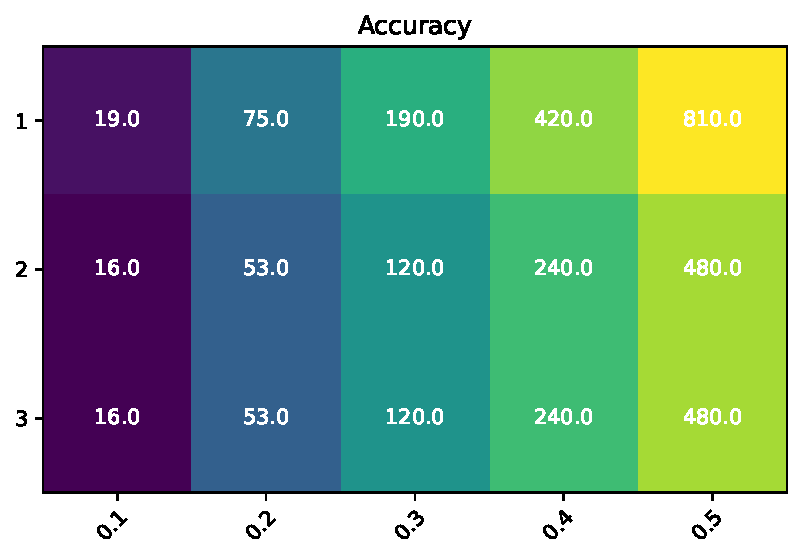
\includegraphics[width=\textwidth]{figures/Accuracy.pdf}
		\caption{Accuracy metric for orthogonal collocation with different size time steps and collocation degrees.}
	\end{subfigure}%
	\hfill
	\begin{subfigure}[b]{0.45\textwidth}
		\centering
		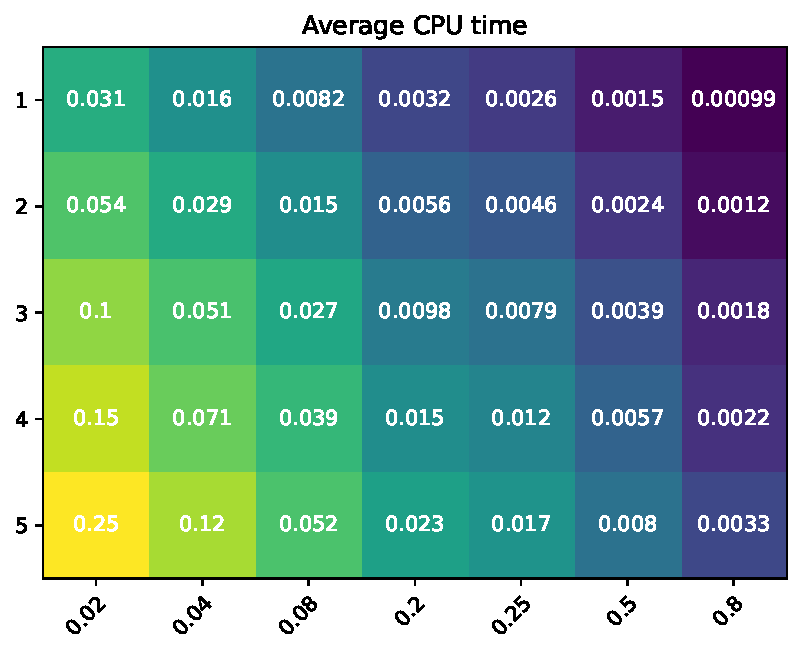
\includegraphics[width=\textwidth]{figures/CPU.pdf}
		\caption{Average CPU time for orthogonal collocation with different size time steps and collocation degrees.}
	\end{subfigure}
	\label{fig:oc}
\end{figure}


\subsection*{Chebyshev Pseudospectral Method}
Multiple shooting is useful for its robustness to discontinuities and nonlinearity and its conceptual simplicity. However, thrust-vectoring dynamics are smooth and continuous, so many of the benefits of multiple shooting are unnecessary. Additionally, multiple shooting introduces a much larger NLP because it solves for the state and control variables at every point in the control horizon. By contrast, Chebyshev Pseudospectral Collocation is a global method that represents the trajectory of each state with a single interpolating polynomial of degree $N$ over the entire horizon, defined by its values at a set of $N+1$ nodes. It achieves spectral accuracy, with error decreasing exponentially as the number of nodes increases, while requiring far fewer decision variables than multiple shooting. For $N=6$ there are seven nodes and $7*13+7*4=119$ decision variables per time step. The dynamics are enforced by constraining the derivative of the interpolant at each node to the dynamic equations. Chebyshev–Gauss–Lobatto nodes are used to cluster more of the nodes towards the beginning and end of the horizon, mitigating the Runge Phenomenon, where polynomial interpolation develops large oscillations near the endpoints. The cosine distribution ensures accuracy and stability:
	\[
        \tau_j = \cos{(\frac{j\pi}{N})},\qquad j = 0,1,...,N
        \]
 These node values are defined from 1 to -1 instead of from time 0 to the end of the horizon. To determine the horizon time for a given tau a linear mapping is used:
         \[
        t(\tau) = \frac{t_f-t_0}{2}\,\tau + \frac{t_f+t_0}{2}, 
        \qquad 
        \frac{dt}{d\tau} = \frac{t_f-t_0}{2}.
        \]
        \[
        \frac{dx}{dt}=\frac{d\tau}{dt}\frac{dx}{d\tau}=\frac{2}{t_f-t_0}\frac{dx}{d\tau}
        \]
At each time step the dynamics are checked with:
        \[
        \frac{dx}{d\tau}(\tau_j) \;\approx\; \sum_{j=0}^N D_{ij}\,x(\tau_j), 
        \qquad i=0,\dots,N.
        \]
Using the chain rule the $\tau$ and time derivatives can be related allowing the node differentiation matrix to be checked against the system dynamics $f(x_i,u_i)$.
        \[
       \dot{x}(t_j)= \frac{2}{t_f-t_0}\sum_{j=0}^N D_{ij}\,x(\tau_j), 
        \]
        \[
        \sum_{j=0}^N D_{ij}\,x_j 
        = \frac{t_f-t_0}{2}\, f(x_i,u_i), 
        \qquad i=1,\dots,N-1.
        \]
Where D is a Chebyshev Differentiation Matrix defined by:
	\[
       D_{N_{00}}=\frac{2N^2+1}{6}
        \]
	\[
       D_{N_{jj}}=\frac{-x_j}{2(1-x_j^2)}
        \]
	\[
       D_{N_{ij}}=\frac{c_i}{c_j}\frac{(-1)^{i+j}}{x_i-x_j}
        \]
	\[
       D_{N_{NN}}=-\frac{2N^2+1}{6}
        \]
	\[
        c_{i/j}=
        \begin{cases}
        2 & i/j = 0 \;\text{or}\; N, \\
        1 & \text{otherwise}.
        \end{cases}
        \]
For $N=6$ the differentiation matrix is:
        \[
        D_{6} =
        \begin{bmatrix}
        \frac{73}{6} & -(8+4\sqrt{3})  & 4 & -2 & \frac{4}{3} & 4\sqrt{3} - 8 & \frac{1}{2}\\
        2+\sqrt{3} & -\sqrt{3} & -(1+\sqrt{3}) & \frac{2}{\sqrt{3}} & 1-\sqrt{3} & \frac{1}{\sqrt{3}} & \frac{1-\sqrt{3}}{1+\sqrt{3}}\\
        -1 & 1+\sqrt{3} & -\frac{1}{3} & -2 & 1 & 1-\sqrt{3} & \frac{1}{3}\\
        \frac{1}{2} & -\frac{2}{\sqrt{3}} & 2 & 0 & -2 & \frac{2}{\sqrt{3}} & -\frac{1}{2}\\
        -\frac{1}{3} & \sqrt{3}-1 & -1 & 2 & \frac{1}{3} & -(1+\sqrt{3}) & 1\\
        \frac{1-\sqrt{3}}{1+\sqrt{3}} & \sqrt{3} & \sqrt{3}-1 & -\frac{2}{\sqrt{3}} & 1+\sqrt{3} & \sqrt{3} &-( 2+\sqrt{3})\\
        -\frac{1}{2} & 8-4\sqrt{3} & -\frac{4}{3} & 2 & -4 & 8+4\sqrt{3} &  -\frac{73}{6}
        \end{bmatrix}
        \]
        
        The chebyshev cost function is:
        	\[
	J=\frac{t_f-t_0}{2}\int_{t_0}^{t_f} \ell(x(t),u(t),t)\,dt \;+\; \phi(x(t_f))
        \]
        \[
        J \;\approx\; \frac{t_f-t_0}{2} \sum_{j=0}^{N} w_j \,\ell(x_j,u_j,t_j)
        \;+\; \phi(x_N),
        \qquad t_j = \frac{t_f-t_0}{2}\,\tau_j + \frac{t_f+t_0}{2}.
        \]
        	
        where $\phi(x(t_f))$ is the terminal cost and  $w_j$ are the Clenshaw-Curtis quadrature weights:

        \[
        w_{\mathrm{j_{even}}} =
        \begin{cases}
        \displaystyle
        \frac{2}{N}\!\left(
        1 - \sum_{n=1}^{\frac{N}{2}-1} \frac{2}{4n^{2}-1}\,
        \cos\!\Big(\tfrac{2 n j \pi}{N}\Big)
        -\frac{(-1)^{j}}{N^{2}-1}
        \right), & 1 \le j \le N-1, \\[2.0ex]
        \displaystyle \frac{1}{N^{2}-1}, & j=0\ \text{or}\ j=N \quad(\text{since \(N\) even}).
        \end{cases}
        \]

	\[
        w_{\mathrm{j_{odd}}} =
        \begin{cases}
        \displaystyle
        \frac{2}{N}\!\left(
        1 - \sum_{n=1}^{\frac{N}{2}-1} \frac{2}{4n^{2}-1}\,
        \cos\!\Big(\tfrac{2 n j \pi}{N}\Big)
        \right), & 1 \le j \le N-1, \\[2ex]
        \displaystyle \frac{1}{N^{2}}, & j=0\ \text{or}\ j=N.
        \end{cases}
        \]

warm starts.
Need to summarize our choices.  Spectral order, time horizon.

\section*{Comparison of Methods}

To compare our different formulations for the NLP problem, we ran a series of simulations each with the drone beginning in a unique and perturbed starting state. In all cases, the drone goal state was to be vertically balanced and motionless at the point $(x,y,z) = (0, 0, 0)$ in three dimensional space. We initially ran a set of seven different simulations. The results for all the simulations were similar in both quality of solutions and timing results, so we present only four of those simulations here.  For each simulation, we computed the average time required to solve the NLP problem at each iteration. The quality of the solutions produced by each method was assessed by comparing the state and control graphs through time. All experiements were run on a Macbook Pro  3.49GHz Apple M2 chip with 8GB RAM. Code was implemented in Python 3.13 using CasADI 3.7.1 \citep{Andersson2018}. 
	
	\subsection*{NLP Solver}
	To solve our non-linear programming (NLP) problems we used the \texttt{ipopt} solver \citep{ipopt} that comes installed with CasADi 3.7.1.  This solver requires an additional subroutine to  solve sparse matrix systems. We experimented with the \texttt{mumps}  solver that comes with CasADi, and also tried using the  \texttt{ma27} and  \texttt{ma57} solvers  from HSL (Harwell Subroutine Library) \citep{hsl}. All solvers were compiled with Apple clang version 17.0.0. The HSL \texttt{ma27} solver produced the most efficient solutions overall. All solvers and experiments were run with the same solver settings.
	\vspace{\baselineskip}
	\begin{python}
        ipopt_settings = {
			'ipopt.max_iter': 100,                  
			'ipopt.tol': 1e-3,                      	
			'ipopt.acceptable_tol': 3e-2,
			'ipopt.linear_solver': 'ma27',
		}
	\end{python}


\subsection*{Results}
We begin with our first simulation which requires the drone to perform a $45^{\circ}$ rotation about the $z$ axis to achieve the goal state. 
Figure (\ref{fig:state45z}) shows a graph of the drone's state overtime for each of our methods: orthagoal collocation, multiple shooter, and Chebyshev pseudospectral. The figures  (\ref{fig:statex1z1vx}), (\ref{fig:statey115dx}) and (\ref{fig:statehover}) show similar graphs for our other three simulations.  Comparison graphs of the control variables are given in figures (\ref{fig:control45z}), (\ref{fig:controlx1z1vx}), (\ref{fig:controly115dx}) and (\ref{fig:controlhover}). Finally, graphs comparing the CPU time for NLP calls throughout the simulations are given in figures (\ref{fig:time45z}), (\ref{fig:timex1z1vx}), (\ref{fig:timey115dx}) and (\ref{fig:timehover}). 
 
\begin{figure}[H]
	\centering
	\begin{subfigure}[b]{0.3\textwidth}
		\centering
		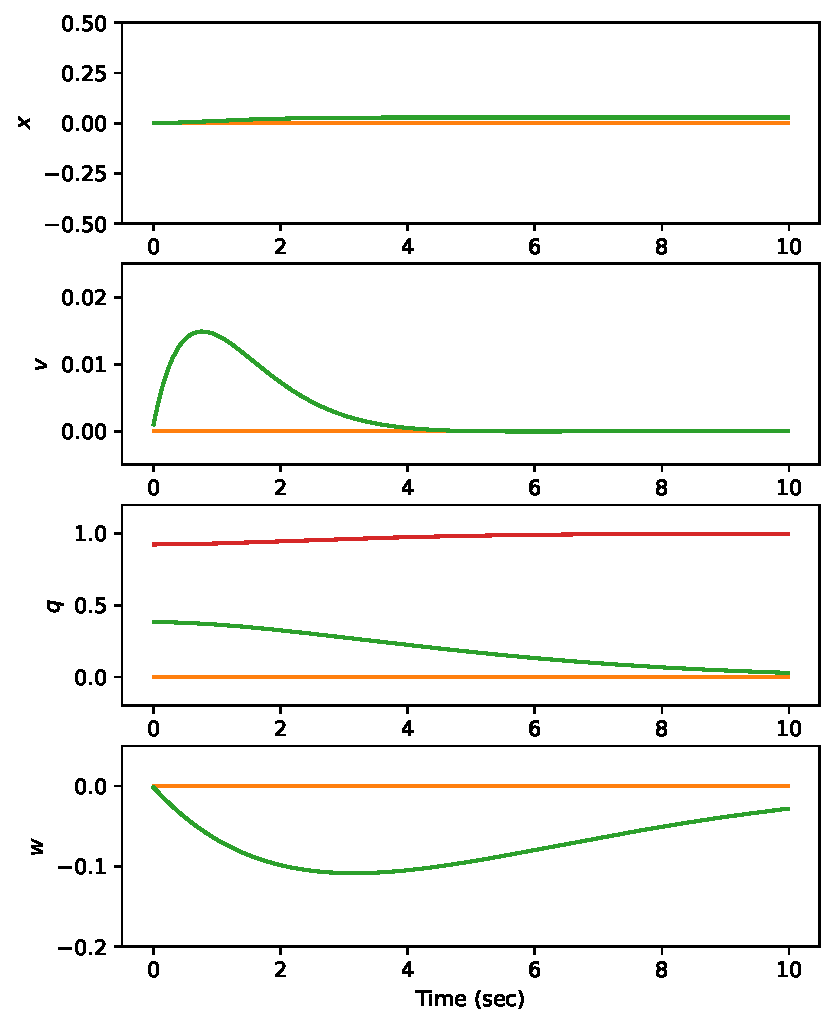
\includegraphics[width=\textwidth]{figures/state45dz1.pdf}
		\caption{orthogonal collocation}
	\end{subfigure}%
	\begin{subfigure}[b]{0.3\textwidth}
		\centering
		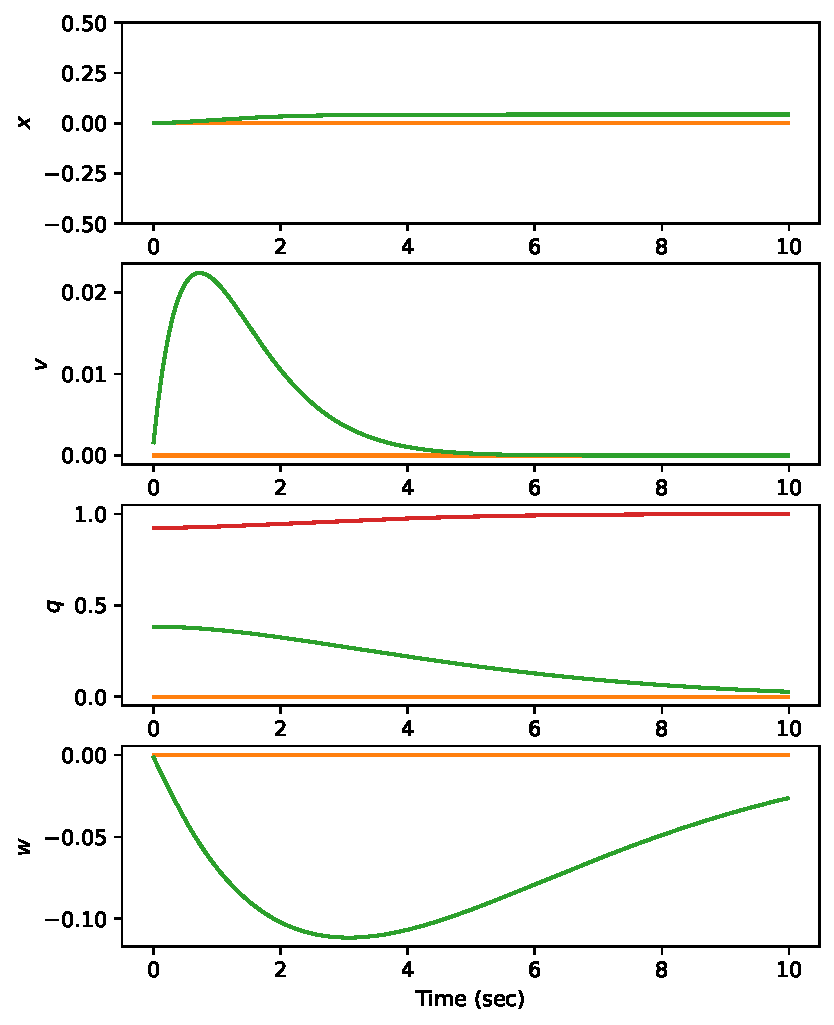
\includegraphics[width=\textwidth]{figures/state45dz3.pdf}
		\caption{multiple shooter}
	\end{subfigure}
	\begin{subfigure}[b]{0.3\textwidth}
		\centering
		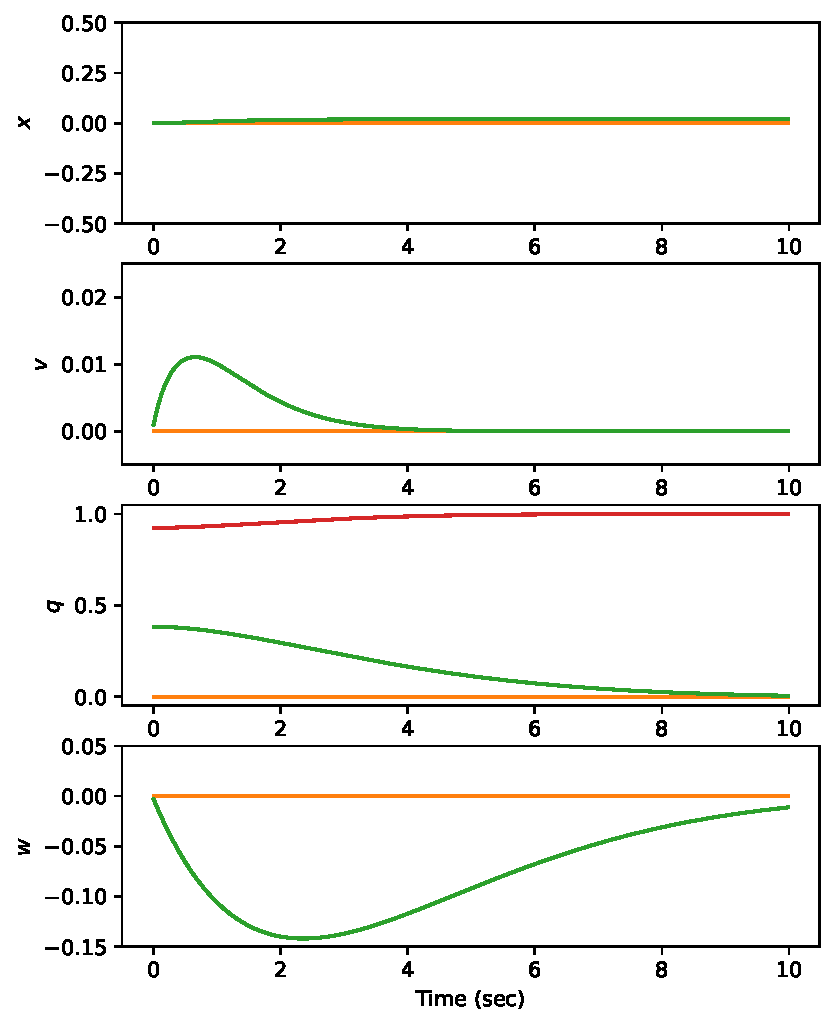
\includegraphics[width=\textwidth]{figures/state45dz2.pdf}
		\caption{Chebyshev pseudospectral}
	\end{subfigure}
	\caption{State data on a simulation requiring a $45^{\circ}$ rotation about the $z$ axis.}
	\label{fig:state45z}
\end{figure}

\begin{figure}[H]
	\centering
	\begin{subfigure}[b]{0.3\textwidth}
		\centering
		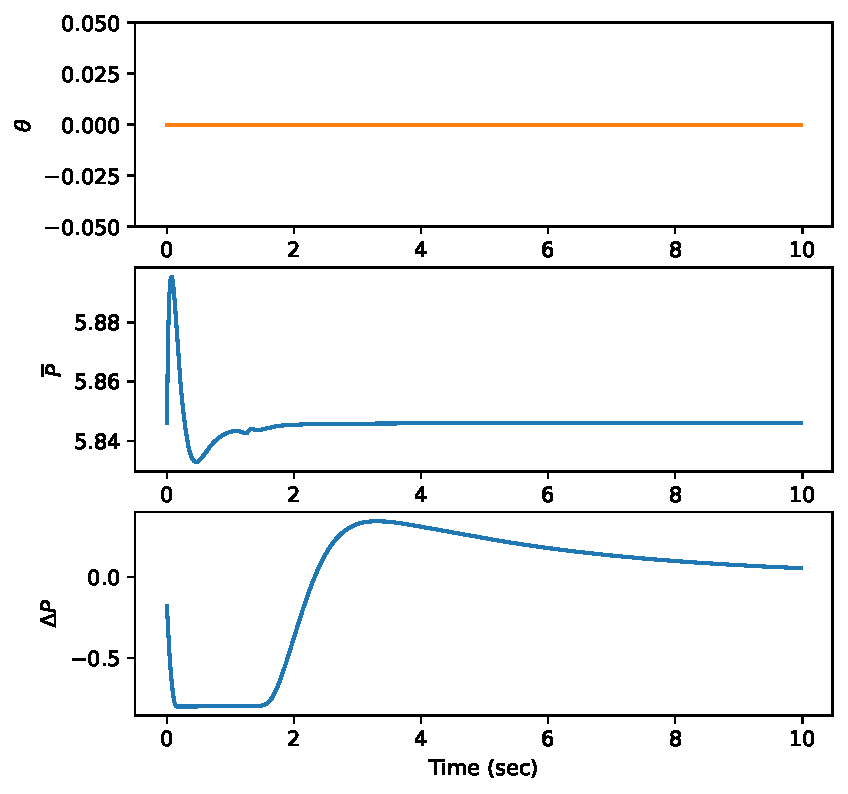
\includegraphics[width=\textwidth]{figures/control45dz4.pdf}
		\caption{orth0gonal collocation}
	\end{subfigure}%
	\begin{subfigure}[b]{0.3\textwidth}
		\centering
		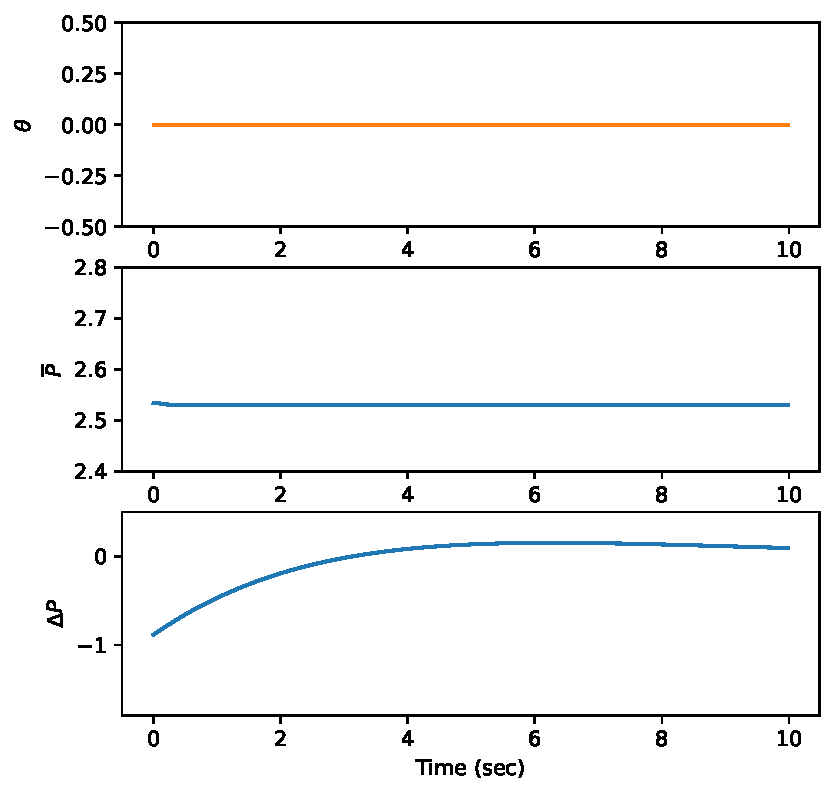
\includegraphics[width=\textwidth]{figures/control45dz6.pdf}
		\caption{multiple shooter}
	\end{subfigure}
	\begin{subfigure}[b]{0.3\textwidth}
		\centering
		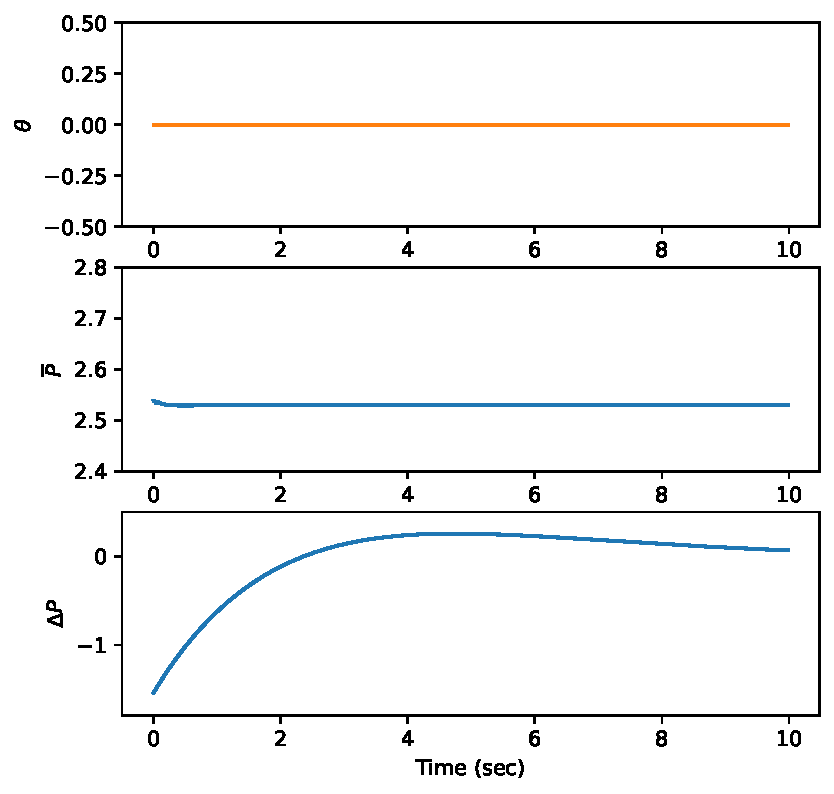
\includegraphics[width=\textwidth]{figures/control45dz5.pdf}
		\caption{Chebyshev pseudospectral}
	\end{subfigure}
	\caption{Control data on a simulation requiring a $45^{\circ}$ rotation about the $z$ axis.}
	\label{fig:control45z}
\end{figure}


\begin{figure}[H]
	\centering
	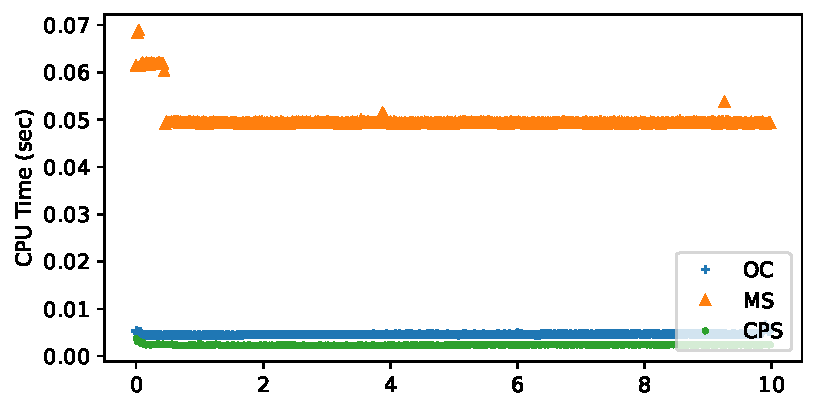
\includegraphics[width=\textwidth]{figures/time45dz.pdf}
	\caption{CPU time for simulation requiring a $45^{\circ}$ rotation about the $z$ axis.}
	\label{fig:time45z}
\end{figure}


\begin{figure}[H]
	\centering
	\begin{subfigure}[b]{0.3\textwidth}
		\centering
		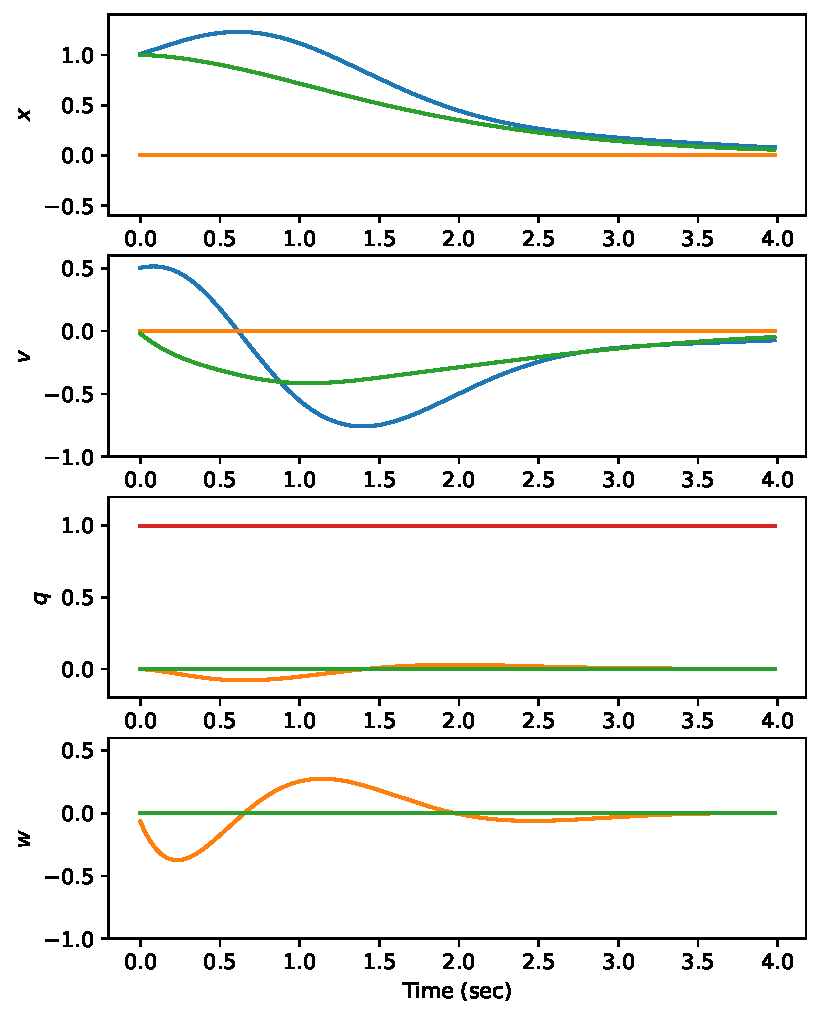
\includegraphics[width=\textwidth]{figures/statex1z1vx1.pdf}
		\caption{orthogonal collocation}
	\end{subfigure}%
	\begin{subfigure}[b]{0.3\textwidth}
		\centering
		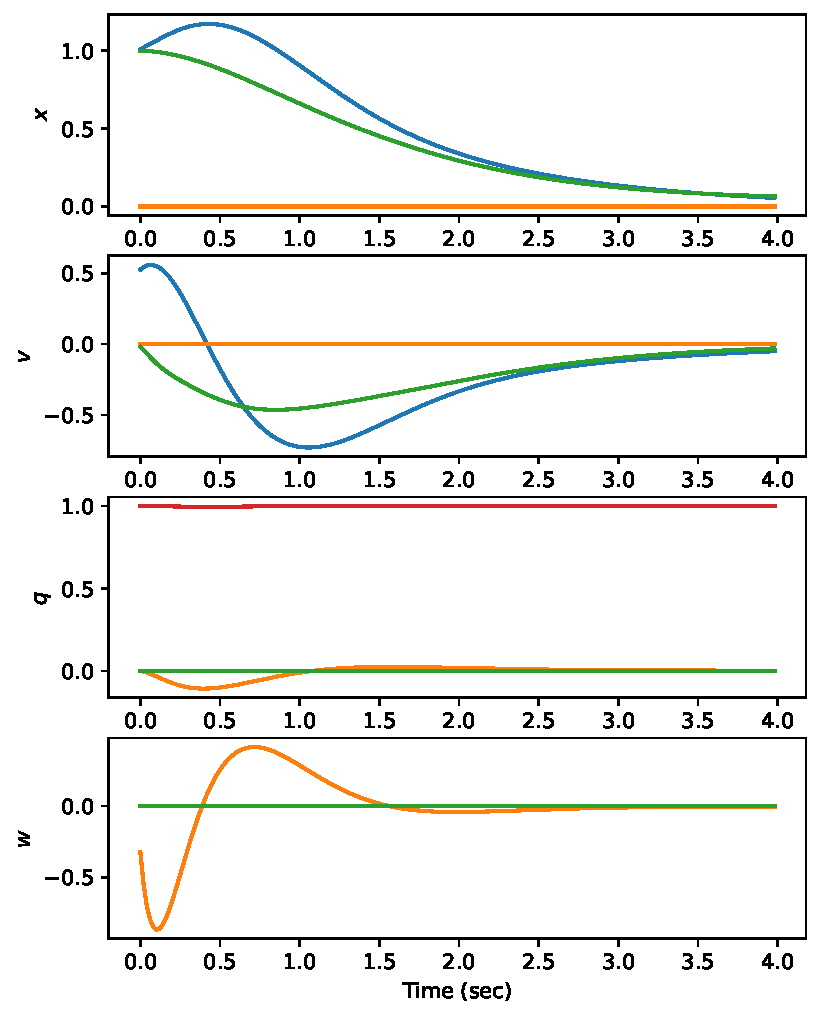
\includegraphics[width=\textwidth]{figures/statex1z1vx3.pdf}
		\caption{multiple shooter}
	\end{subfigure}
	\begin{subfigure}[b]{0.3\textwidth}
		\centering
		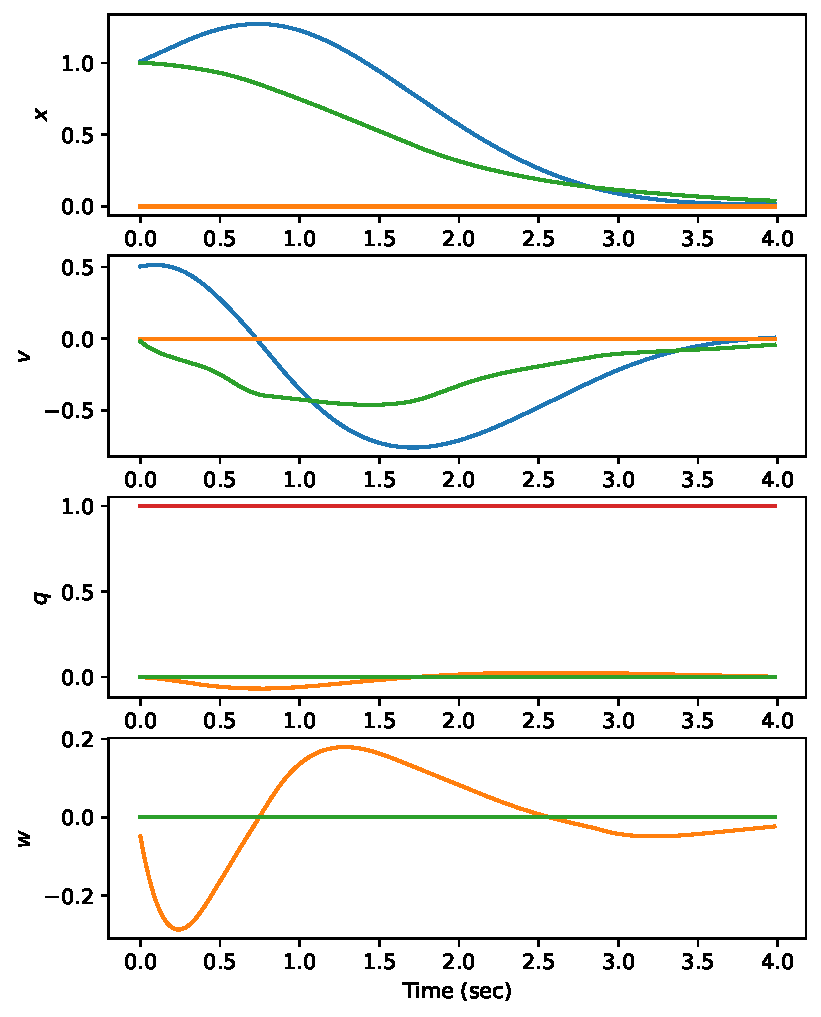
\includegraphics[width=\textwidth]{figures/statex1z1vx2.pdf}
		\caption{Chebyshev pseudospectral}
	\end{subfigure}
	\caption{State data on a simulation with initial conditions: $x = 1$, $z=1$, $v_x = 0.5$ }
	\label{fig:statex1z1vx}
\end{figure}

\begin{figure}[H]
	\centering
	\begin{subfigure}[b]{0.3\textwidth}
		\centering
		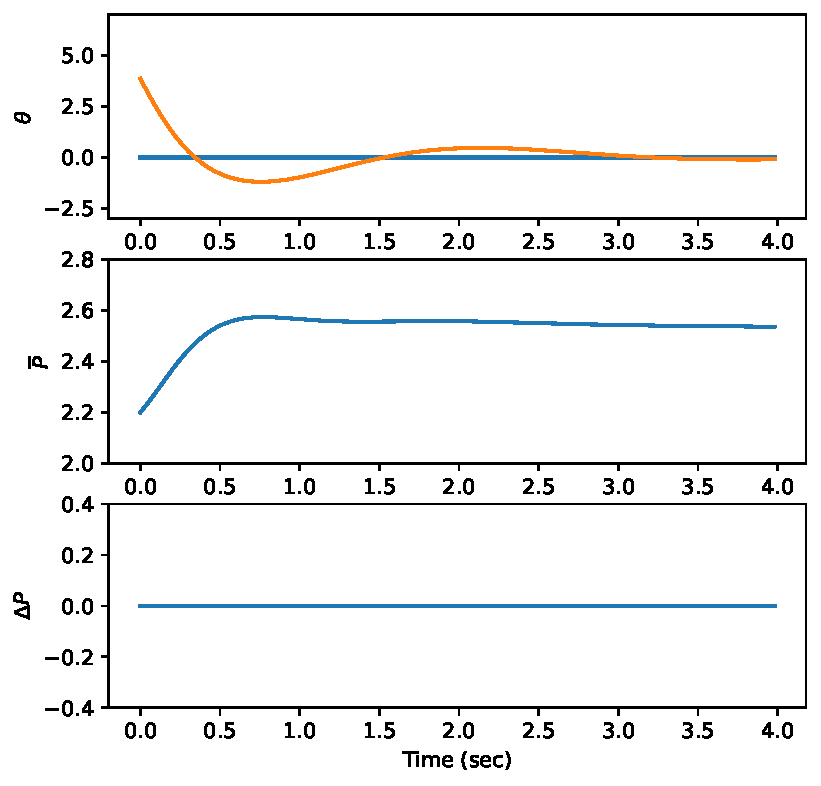
\includegraphics[width=\textwidth]{figures/controlx1z1vx4.pdf}
		\caption{orthogonal collocation}
	\end{subfigure}%
	\begin{subfigure}[b]{0.3\textwidth}
		\centering
		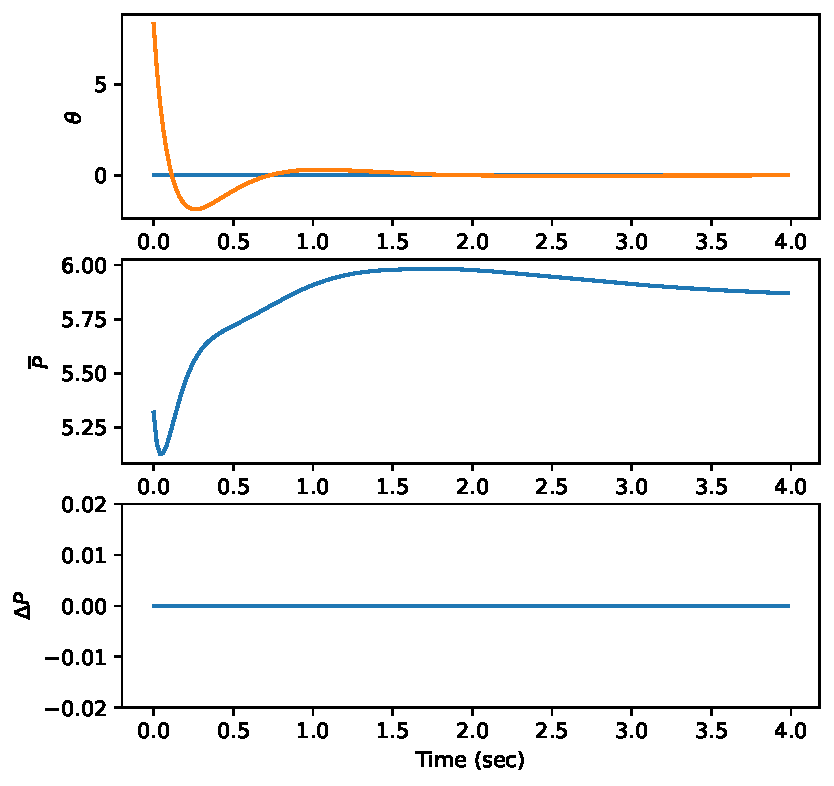
\includegraphics[width=\textwidth]{figures/controlx1z1vx6.pdf}
		\caption{multiple shooter}
	\end{subfigure}
	\begin{subfigure}[b]{0.3\textwidth}
		\centering
		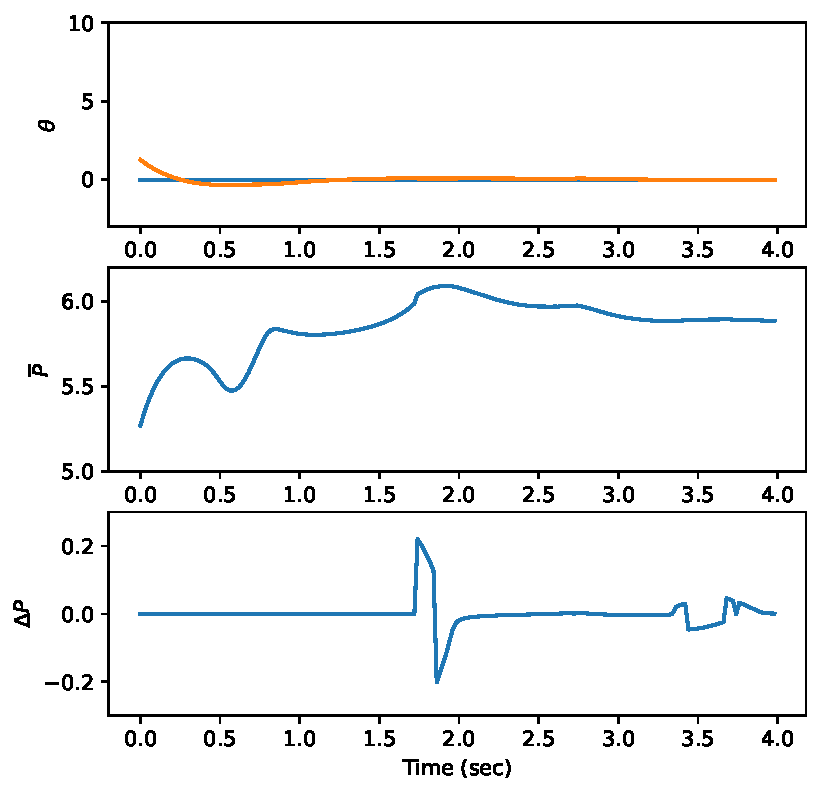
\includegraphics[width=\textwidth]{figures/controlx1z1vx5.pdf}
		\caption{Chebyshev pseudospectral}
	\end{subfigure}
	\caption{Control data on a simulation with initial conditions: $x = 1$, $z=1$, $v_x = 0.5$}
	\label{fig:controlx1z1vx}
\end{figure}


\begin{figure}[H]
	\centering
	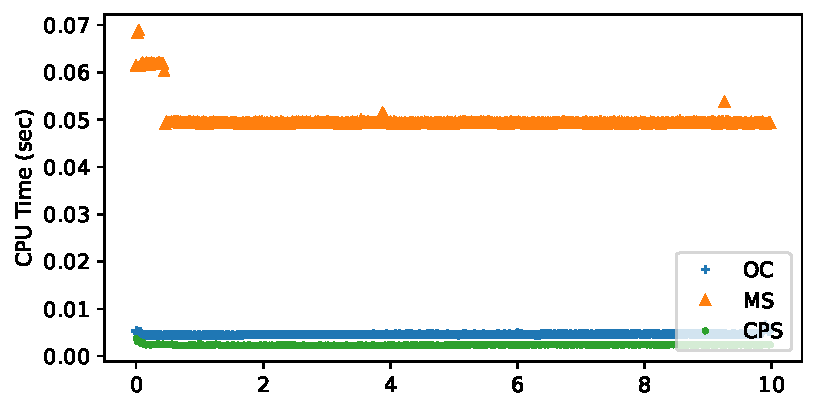
\includegraphics[width=\textwidth]{figures/time45dz.pdf}
	\caption{CPU time for a simulation with initial conditions: $x = 1$, $z=1$, $v_x = 0.5$}
	\label{fig:timex1z1vx}
\end{figure}

\begin{figure}[H]
	\centering
	\begin{subfigure}[b]{0.3\textwidth}
		\centering
		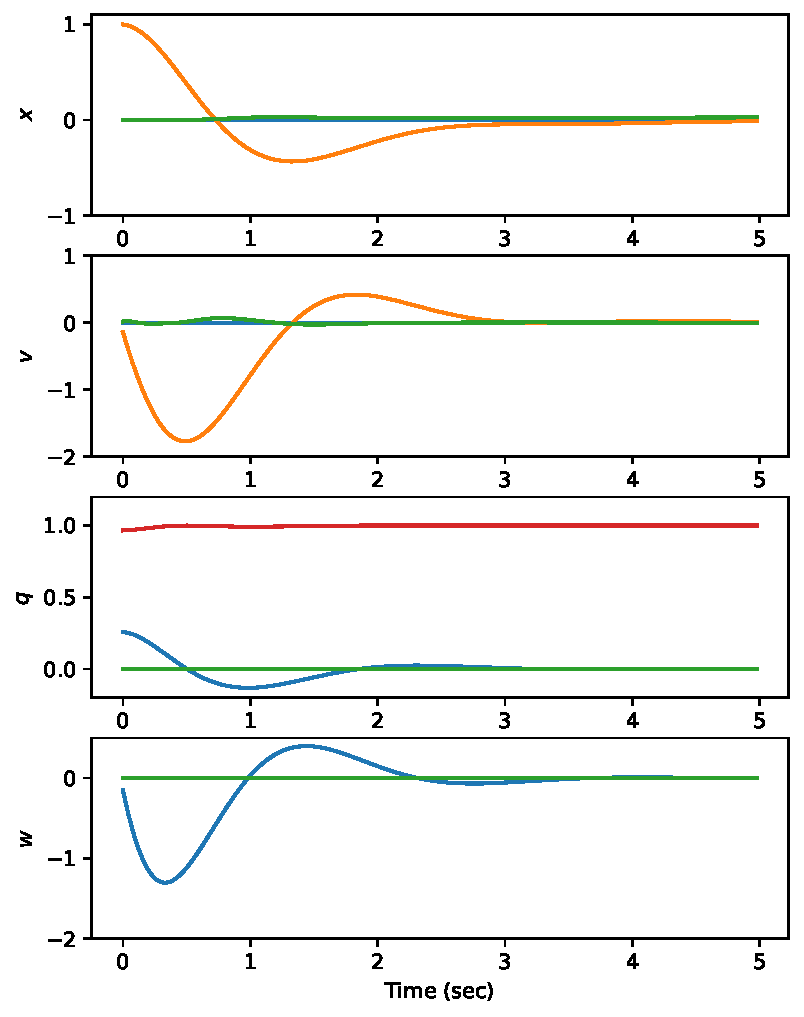
\includegraphics[width=\textwidth]{figures/statey115dx1.pdf}
		\caption{orthogonal collocation}
	\end{subfigure}%
	\begin{subfigure}[b]{0.3\textwidth}
		\centering
		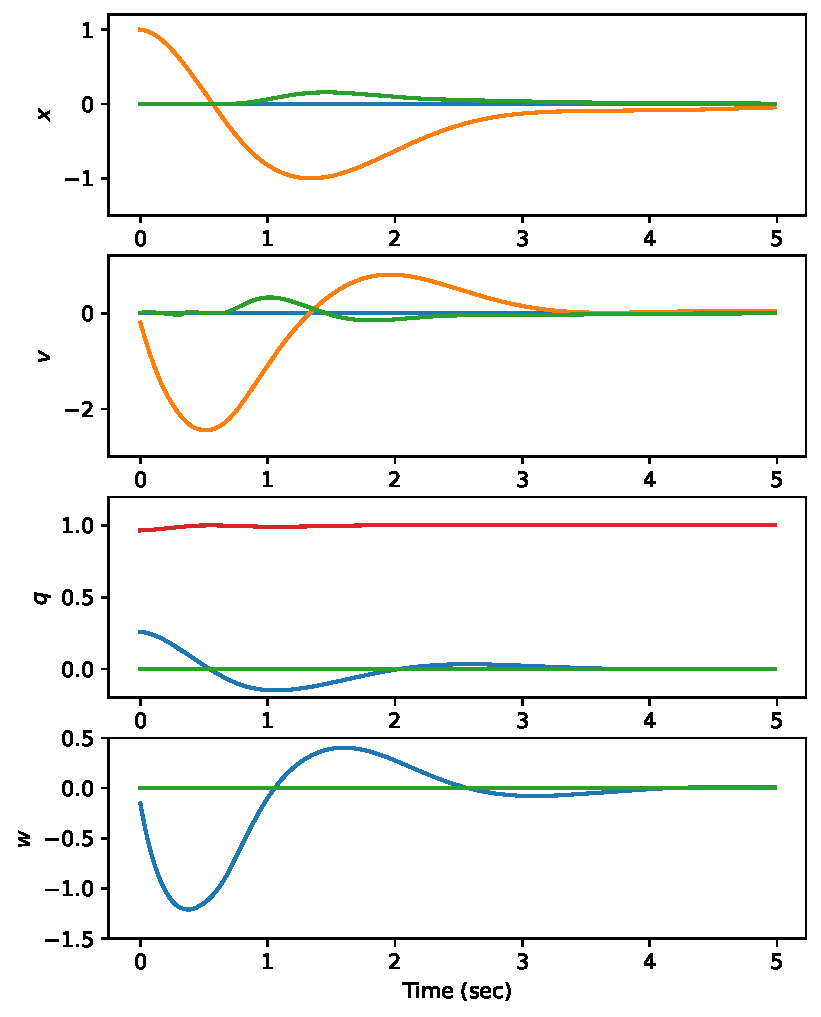
\includegraphics[width=\textwidth]{figures/statey115dx3.pdf}
		\caption{multiple shooter}
	\end{subfigure}
	\begin{subfigure}[b]{0.3\textwidth}
		\centering
		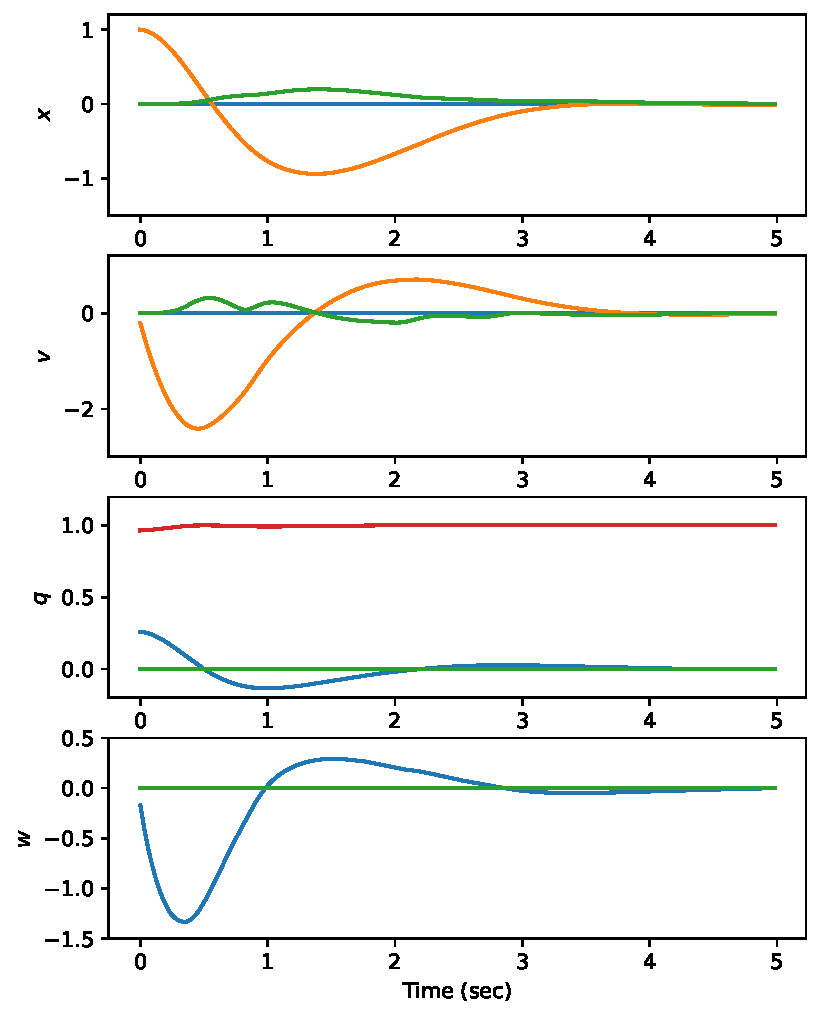
\includegraphics[width=\textwidth]{figures/statey115dx2.pdf}
		\caption{Chebyshev pseudospectral}
	\end{subfigure}
	\caption{State data on a simulation with initial conditions: $y = 1$,$15^{\circ}$ rotation about $x$ axis.}
	\label{fig:statey115dx}
\end{figure}

\begin{figure}[H]
	\centering
	\begin{subfigure}[b]{0.3\textwidth}
		\centering
		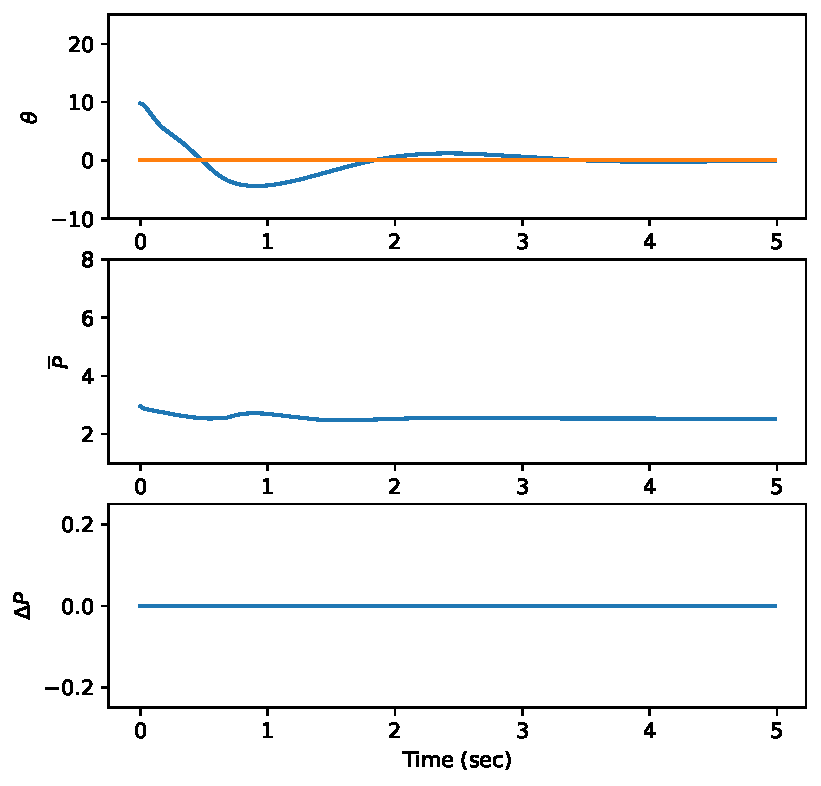
\includegraphics[width=\textwidth]{figures/controly115dx4.pdf}
		\caption{orthogonal collocation}
	\end{subfigure}%
	\begin{subfigure}[b]{0.3\textwidth}
		\centering
		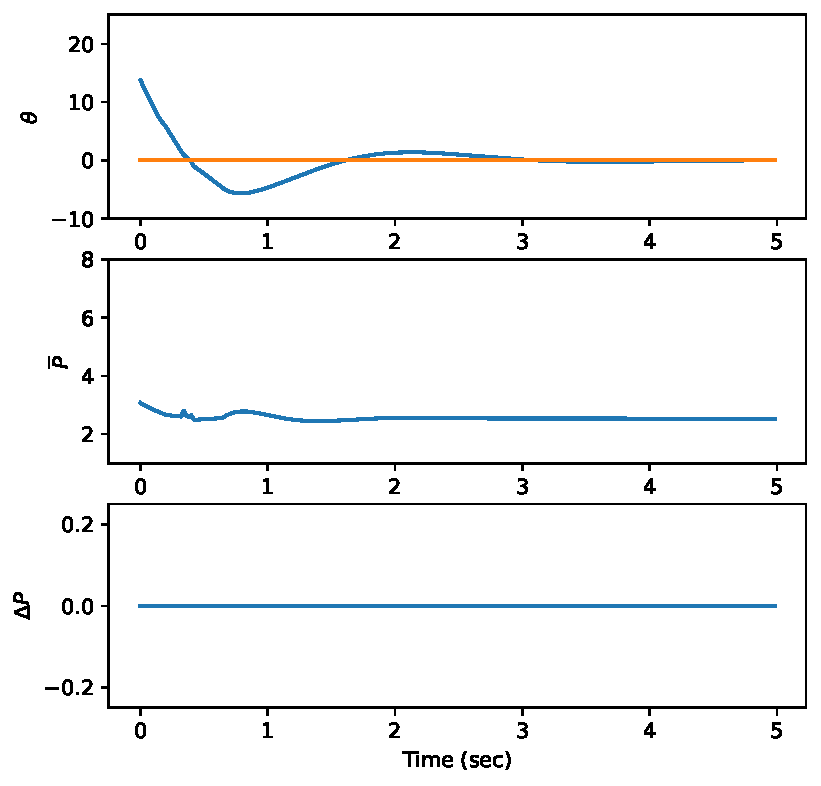
\includegraphics[width=\textwidth]{figures/controly115dx6.pdf}
		\caption{multiple shooter}
	\end{subfigure}
	\begin{subfigure}[b]{0.3\textwidth}
		\centering
		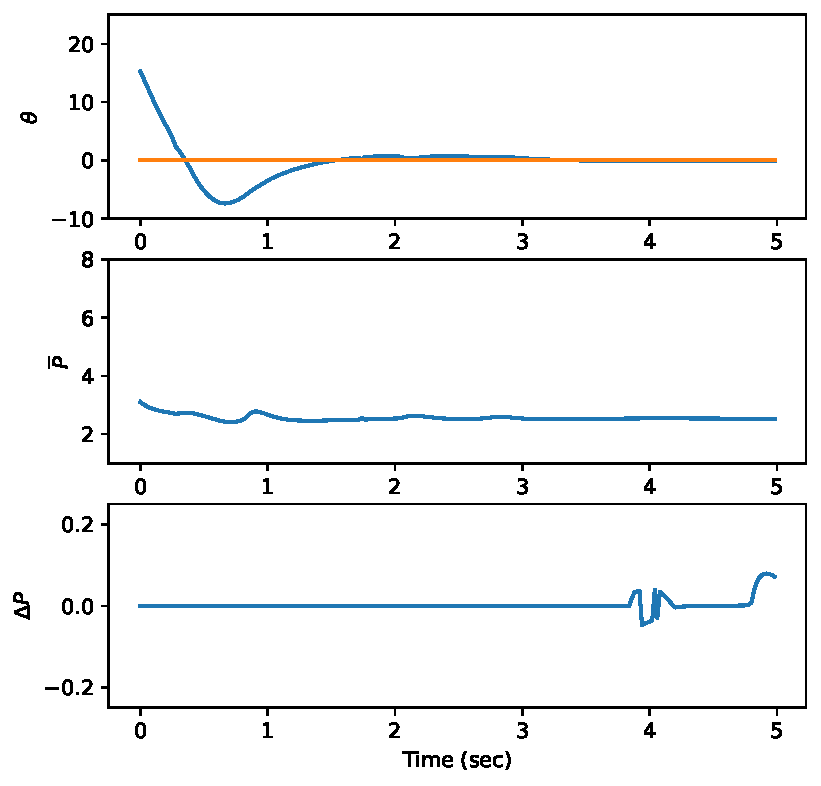
\includegraphics[width=\textwidth]{figures/controly115dx5.pdf}
		\caption{Chebyshev pseudospectral}
	\end{subfigure}
	\caption{Control data on a simulation with initial conditions: $y = 1$,$15^{\circ}$ rotation about $x$ axis.}
	\label{fig:controly115dx}
\end{figure}


\begin{figure}[H]
	\centering
	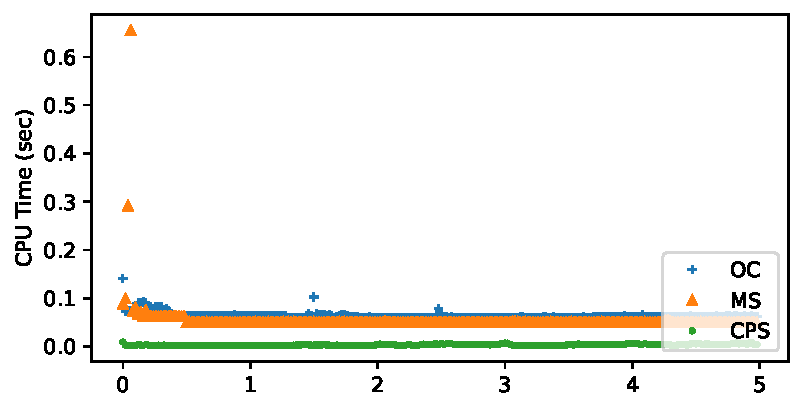
\includegraphics[width=\textwidth]{figures/timey115dx.pdf}
	\caption{CPU time for simulation with initial conditions: $y = 1$,$15^{\circ}$ rotation about $x$ axis.}
	\label{fig:timey115dx}
\end{figure}




\begin{figure}[H]
	\centering
	\begin{subfigure}[b]{0.3\textwidth}
		\centering
		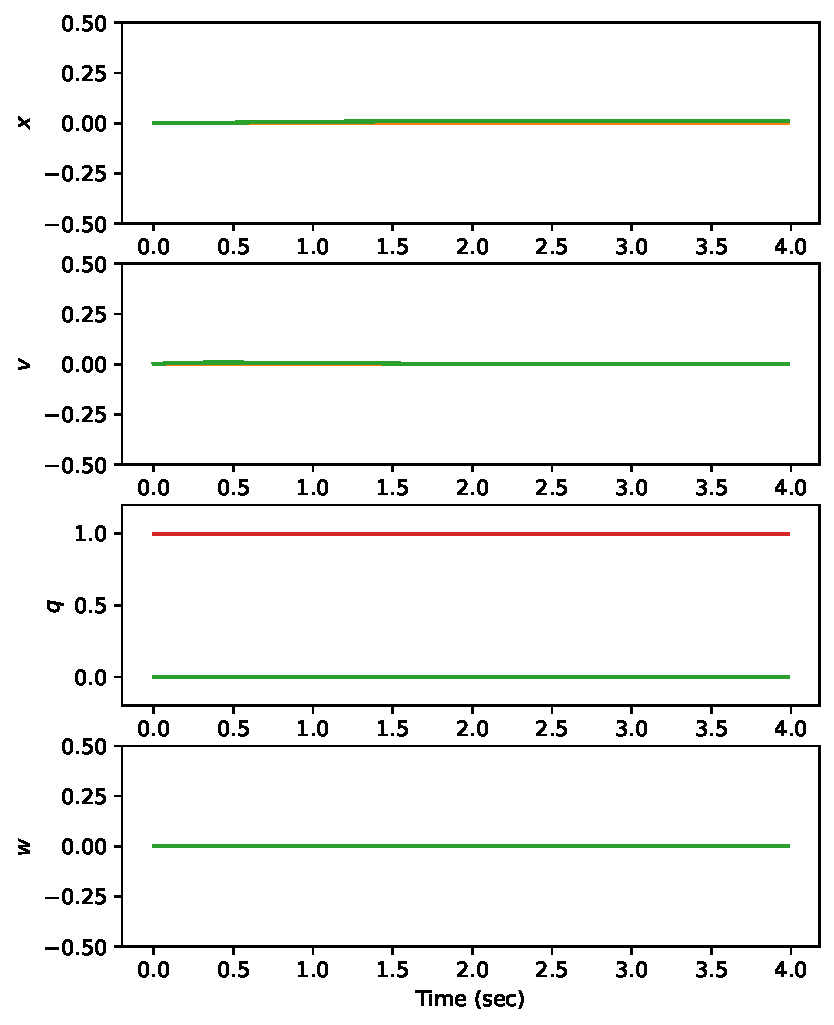
\includegraphics[width=\textwidth]{figures/statehover1.pdf}
		\caption{orthogonal collocation}
	\end{subfigure}%
	\begin{subfigure}[b]{0.3\textwidth}
		\centering
		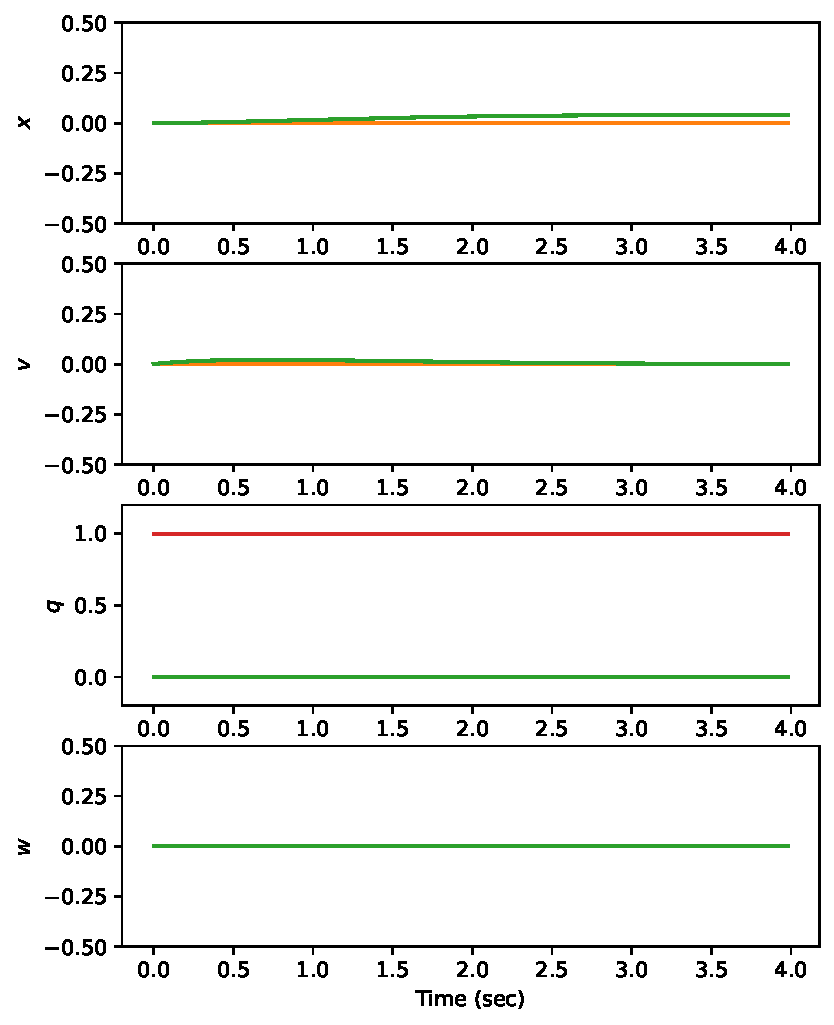
\includegraphics[width=\textwidth]{figures/statehover3.pdf}
		\caption{multiple shooter}
	\end{subfigure}
	\begin{subfigure}[b]{0.3\textwidth}
		\centering
		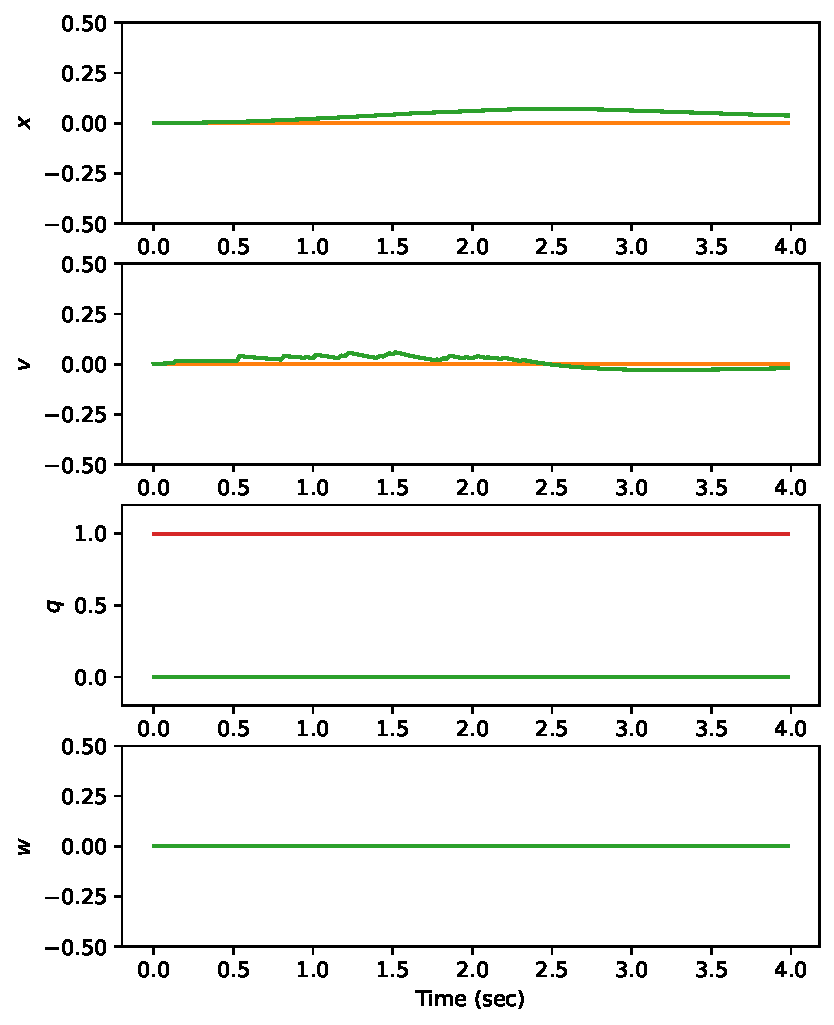
\includegraphics[width=\textwidth]{figures/statehover2.pdf}
		\caption{Chebyshev pseudospectral}
	\end{subfigure}
	\caption{State data on a simulation with initial state equal to goal state.}
	\label{fig:statehover}
\end{figure}

\begin{figure}[H]
	\centering
	\begin{subfigure}[b]{0.3\textwidth}
		\centering
		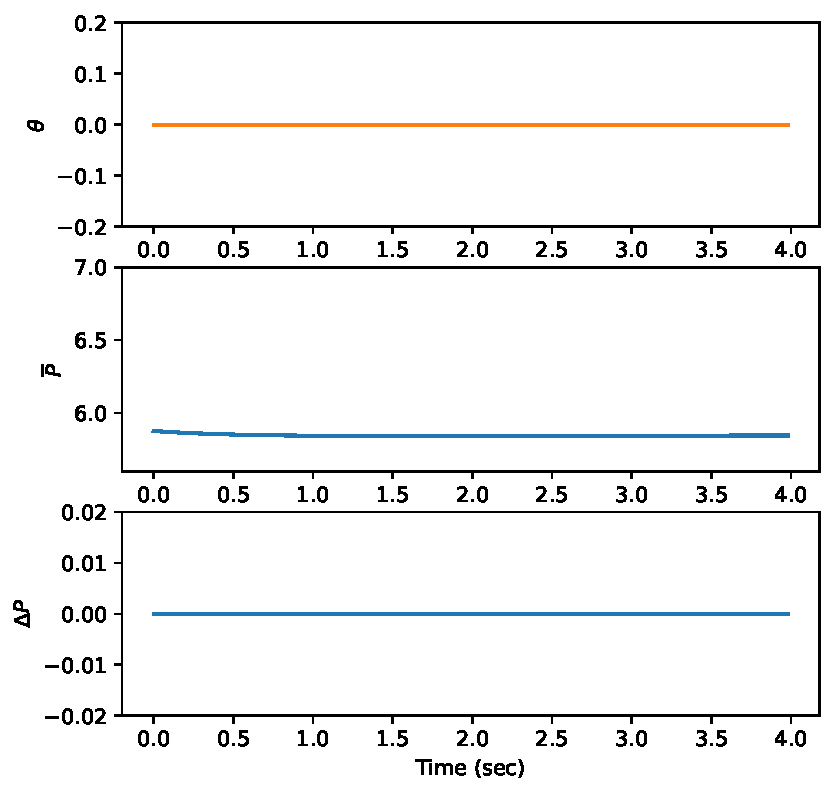
\includegraphics[width=\textwidth]{figures/controlhover4.pdf}
		\caption{orthogonal collocation}
	\end{subfigure}%
	\begin{subfigure}[b]{0.3\textwidth}
		\centering
		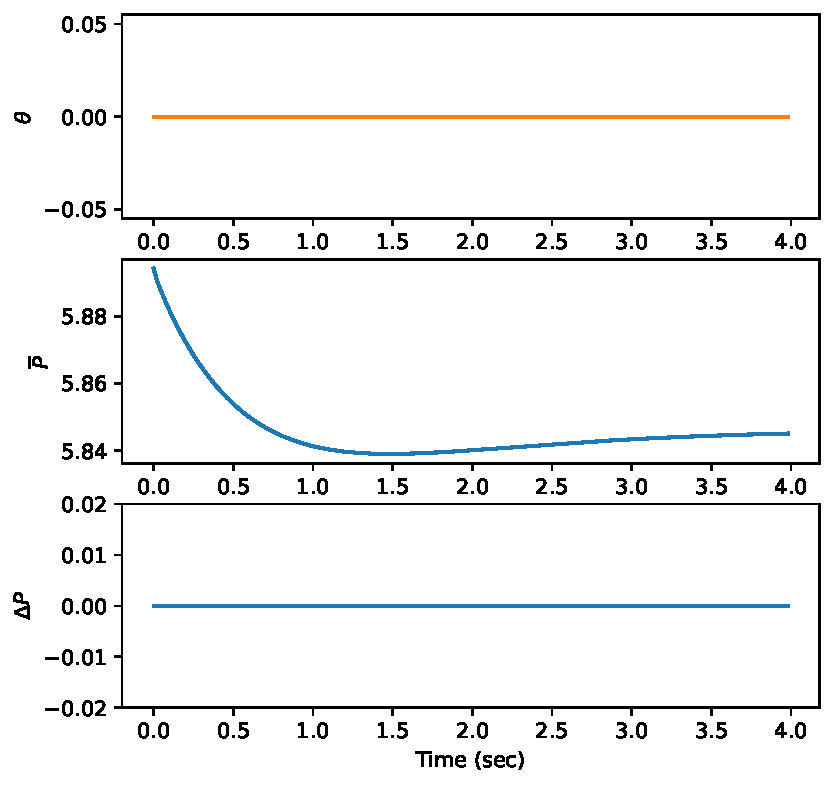
\includegraphics[width=\textwidth]{figures/controlhover6.pdf}
		\caption{multiple shooter}
	\end{subfigure}
	\begin{subfigure}[b]{0.3\textwidth}
		\centering
		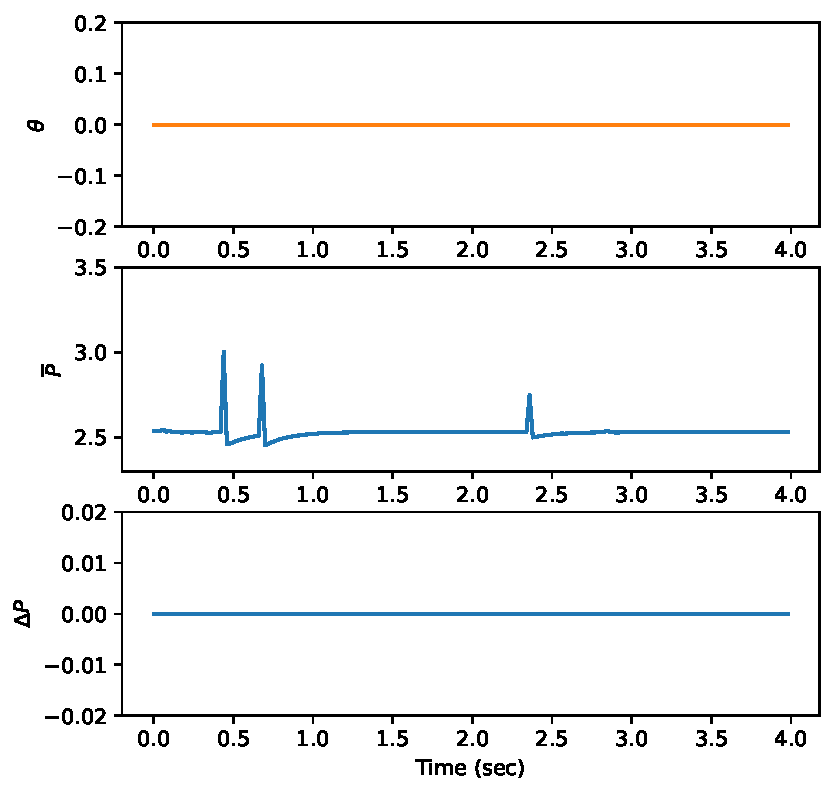
\includegraphics[width=\textwidth]{figures/controlhover5.pdf}
		\caption{Chebyshev pseudospectral}
	\end{subfigure}
	\caption{Control data on a simulation with initial state equal to goal state.}
	\label{fig:controlhover}
\end{figure}


\begin{figure}[H]
	\centering
	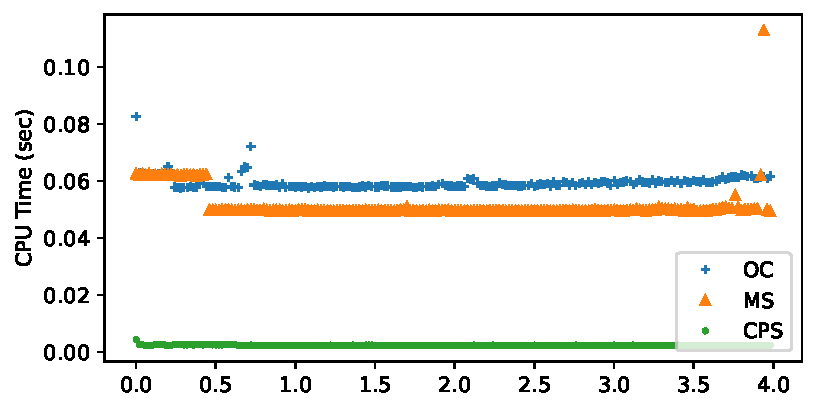
\includegraphics[width=\textwidth]{figures/timehover.pdf}
	\caption{CPU time for simulation with initial state equal to goal state.}
	\label{fig:timehover}
\end{figure}


All of the methods provide good quality solutions with state values that behaved smoothly and converged to the desired goal state. The graphs of control variables were generally smooth, but all methods occasionally constructed solutions where the  average thrust $\overline{P}$ seemed more irregular than required to reach the goal state.  Real world experiments on the drone will be needed to determine if solutions with these irregularities will negatively affect performance in practice.


\begin{table}[h!]	
	\begin{center}
		\begin{tabular}{ | l | c | c | c | } 
			\hline
			initial state & OC  & MS & CPS \\
			\hline
			$45^{\circ}$ rotation about $z$ axis & 0.063 &       0.056 & 0.002 \\ 
			$x = 1$, $z=1$, $v_x = 0.5$  & 0.059          &        0.046 & 0.003 \\ 
			$y = 1$,$15^{\circ}$ rotation about $x$ axis &0.063          &       0.06 & 0.004\\ 
				initial state equal to goal state & 0.062    &            0.056  & 0.002 \\ 
			\hline
		\end{tabular}
		\caption{Comparison of average CPU time in seconds for solution of NLP for a series of  simulations. Methods include orthogonal collocation (OC),  multiple shooter (MS), and Chebyshev pseudospectral method (CPS). }
		\label{table:CPU}
	\end{center}

\end{table}

 Our goal is to run our control algorithm at $50$Hz on the Raspberry Pi 5. The CPU speed of the Pi is 2.4GHz while our experiments were run on a machine with a CPU speed of 3.49GHz. To meet our goal of 50Hz on the Pi we need a solution time on the experiment machine of less than $0.014$ seconds. Table (\ref{table:CPU}) summarizes the average CPU time for solution of the NLP problem for each simulation and each method.  The run times for the orthogonal collocation and multiple shooter are both too slow to meet our  $50$Hz target.  Additional changes such as reducing the length of the horizon or relaxing convergence criteria might improve these times somewhat, but they are unlikely to provide the performance needed for this application of NMPC.  The Chebyshev pseudospectral method is substantially faster and comfortably meets our $0.014$ solution time while providing solution graphs with comparable quality.

\section*{Conclusions}
We implemented three different formulations of the NPL problem for an NMPC algorithm controlling a thrust vector drone and compared their solution quality and relative efficiency. All methods produced good quality solutions while only the Chebyshev pseudospectral method provided solutions that are efficient enough to control the drone on a Raspberry Pi 5. Further real-world experiments are required to determine if the solutions produced provide good control in practice.
	
	
%	\nocite{*}
%	

\bibliography{references.bib}
\end{document}

